\documentclass[smallextended]{svjour3}\usepackage[]{graphicx}\usepackage[]{color}
%% maxwidth is the original width if it is less than linewidth
%% otherwise use linewidth (to make sure the graphics do not exceed the margin)
\makeatletter
\def\maxwidth{ %
  \ifdim\Gin@nat@width>\linewidth
    \linewidth
  \else
    \Gin@nat@width
  \fi
}
\makeatother

\definecolor{fgcolor}{rgb}{0.345, 0.345, 0.345}
\newcommand{\hlnum}[1]{\textcolor[rgb]{0.686,0.059,0.569}{#1}}%
\newcommand{\hlstr}[1]{\textcolor[rgb]{0.192,0.494,0.8}{#1}}%
\newcommand{\hlcom}[1]{\textcolor[rgb]{0.678,0.584,0.686}{\textit{#1}}}%
\newcommand{\hlopt}[1]{\textcolor[rgb]{0,0,0}{#1}}%
\newcommand{\hlstd}[1]{\textcolor[rgb]{0.345,0.345,0.345}{#1}}%
\newcommand{\hlkwa}[1]{\textcolor[rgb]{0.161,0.373,0.58}{\textbf{#1}}}%
\newcommand{\hlkwb}[1]{\textcolor[rgb]{0.69,0.353,0.396}{#1}}%
\newcommand{\hlkwc}[1]{\textcolor[rgb]{0.333,0.667,0.333}{#1}}%
\newcommand{\hlkwd}[1]{\textcolor[rgb]{0.737,0.353,0.396}{\textbf{#1}}}%

\usepackage{framed}
\makeatletter
\newenvironment{kframe}{%
 \def\at@end@of@kframe{}%
 \ifinner\ifhmode%
  \def\at@end@of@kframe{\end{minipage}}%
  \begin{minipage}{\columnwidth}%
 \fi\fi%
 \def\FrameCommand##1{\hskip\@totalleftmargin \hskip-\fboxsep
 \colorbox{shadecolor}{##1}\hskip-\fboxsep
     % There is no \\@totalrightmargin, so:
     \hskip-\linewidth \hskip-\@totalleftmargin \hskip\columnwidth}%
 \MakeFramed {\advance\hsize-\width
   \@totalleftmargin\z@ \linewidth\hsize
   \@setminipage}}%
 {\par\unskip\endMakeFramed%
 \at@end@of@kframe}
\makeatother

\definecolor{shadecolor}{rgb}{.97, .97, .97}
\definecolor{messagecolor}{rgb}{0, 0, 0}
\definecolor{warningcolor}{rgb}{1, 0, 1}
\definecolor{errorcolor}{rgb}{1, 0, 0}
\newenvironment{knitrout}{}{} % an empty environment to be redefined in TeX

\usepackage{alltt}       % onecolumn (second format)
\RequirePackage{fix-cm}
\smartqed% flush right qed marks, e.g. at end of proof
\usepackage{graphicx}
\usepackage[round]{natbib}
\IfFileExists{upquote.sty}{\usepackage{upquote}}{}
\begin{document}
\journalname{Computational Statistics}
\title{Community engagement and subgroup meta-knowledge: Some factors in the soul of a community}


\titlerunning{Community engagement and subgroup meta-knowledge}        % if too long for running head

\author{Amelia McNamara}
\institute{A. McNamara \at
              8125 Math Sciences Bldg. \\
              Los Angeles, CA 90095-1554 \\
              \email{amelia.mcnamara@stat.ucla.edu}
}

\date{Received: date / Accepted: date}
\maketitle



\begin{abstract} The Knight Foundation collects data to determine what factors impact community satisfaction, local GDP growth, and interest in Knight news publications. For the 2013 Data Expo at the Joint Statistical Meetings, many participants created graphical explorations of these data. This article focuses on the idea of community meta-knowledge, which is essentially majority group empathy or understanding of how minorities experience their community. For example, the survey asks participants to rate their community ``as a place for senior citizens,'' on a 5-point Likert scale. A city where seniors rated their community in the same way as non-seniors is defined as a community with high meta-knowledge about conditions for seniors. Three minority groups were explored: seniors, families with young children, and racial minorities. In most communities, people outside the minority group tended to under-rate their community, compared to those in the minority group. However, there were some exceptions. 
\keywords{2013 Data Exposition, R, ggplot2, Likert scales, meta-knowledge}
\end{abstract}

\section{Introduction}
\label{intro}
Studies have shown that increasing empathy is the best way to improve intergroup relations \citep{SteFin1999}. Therefore, it is of interest to quantify the typical level of empathy in communities across the United States. The Knight Foundation data provides a window to a factor which could be thought of as a proxy for empathy, namely community meta-knowledge. We are defining meta-knowledge as community awareness by those outside a specific subgroup about the conditions for people inside the subgroup. The primary attempt of this article is to answer the question ``Are people outside a specific subgroup aware of the quality of their community for people in that subgroup?" and then, ``do communities with high meta-knowledge (those where people outside the subgroup understood conditions for minorities) have higher community satisfaction rates than those with low meta-knowledge?"

This article is one of several related to the Knight Foundation community data from the 2013 Data Expo. For more information on the Expo and the data sets, see \citep{HofWic20XX}.

\section{The Data}
\label{data}
The Knight Foundation collects survey data on 26 communities where the Knight brothers own newspapers, including San Jose, CA, State College, PA, Palm Beach, FL, and St. Paul, MN. The foundation provided data for three years, starting in 2008. Each data set includes approximately 20 demographic questions and 50-80 survey questions, depending on how distinct questions are defined. The aim of the survey is to gauge what factors are important to community attachment, and it includes questions on a variety of subjects, from ``how satisfied are you with this community as a place to live?" to ``how many minutes is your daily commute?"

The survey is conducted over the phone by Gallup Poll, and can take place in either English or Spanish. Gallup also performs data analysis for the Knight Foundation, and their yearly reports are available on the Knight Foundation website \citep{KF2008, KF2009, KF2010}. 

The existing data analysis from Gallup is related to a metric they call ``Community Attachment." It is difficult to pin down what this variable means, but it's a composite metric composed of Community Loyalty and Community Passion. Both of those metrics, in turn, are composed of several variables. Community Loyalty includes how likely a person says they are to stay in that particular area, how much they would recommend it to friends, and their outlook for the community's future \citep{KF2010}. Community Passion is composed of variables on connectedness and community pride. So, Community Attachment is already a model of what Gallup believes is important to strong communities. The Gallup team has discovered that this composite variable is positively correlated with local Gross Domestic Product (GDP) growth \citep{KF2010b}. Because of this relationship, the analysis from Gallup is focused on what other factors correlate with Community Attachment (and therefore, with local GDP growth). 

While the Gallup Poll analysis is interesting, it does raise the question of multicollinearity, as factors that are correlated with Community Attachment may simply be correlated with one of the variables that was used to compose it, and may not actually have an impact on local GDP growth. 













\subsection{Community Survey Rates}
\label{maprates}



\begin{knitrout}
\definecolor{shadecolor}{rgb}{0.969, 0.969, 0.969}\color{fgcolor}\begin{figure}

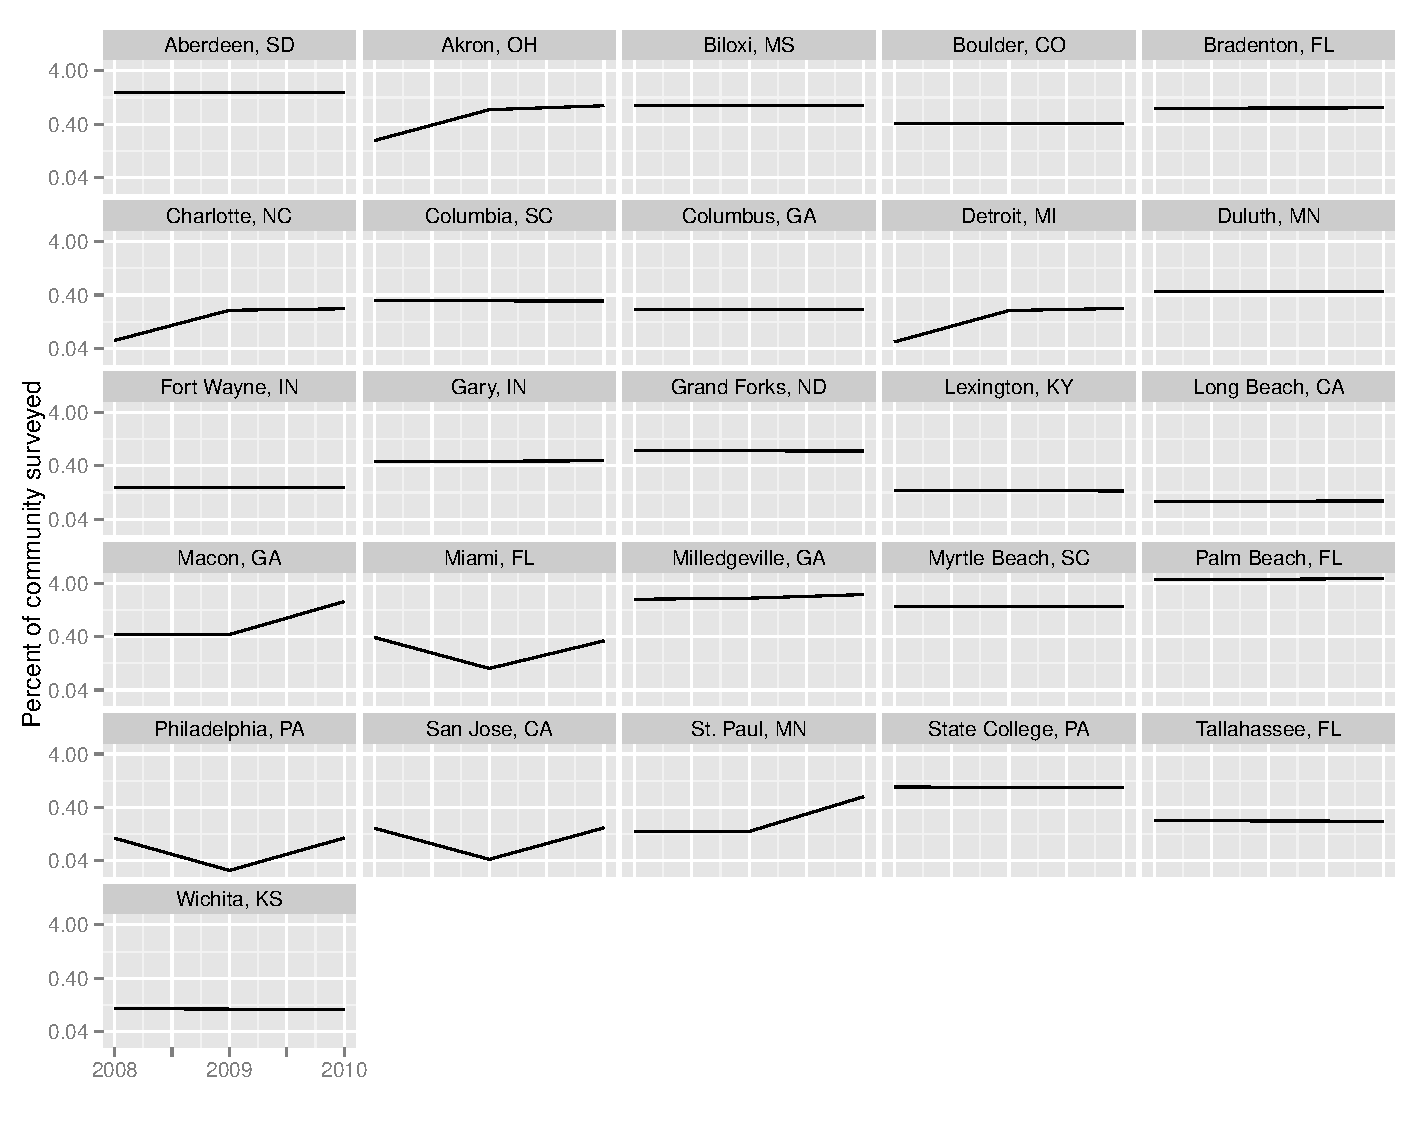
\includegraphics[width=0.99\linewidth]{surveyrates-1} \hfill{}

\caption[Yearly survey percentages, displayed on a log scale]{Yearly survey percentages, displayed on a log scale. Notice that some communities are always over-surveyed (for example, Palm Beach, FL) and some always appear under-surveyed (for example, Long Beach, CA). Population data compiled by the Census Bureau for Intercensal population estimates}\label{fig:surveyrates}
\end{figure}


\end{knitrout}
As mentioned above, the data were collected by Gallup through telephone surveys in 2008, 2009, and 2010. Participants were a random sample of adults living in 26 ``communities" (cities or metro areas of the United States). The data from 2008 and 2009 had 13822 and 13728 responses, respectively, while the data from 2010 contained 20271 observations. Because the data sets surveyed the same 26 communities, we can calculate the average number of survey participants in each community. In 2008, that average was 531 people, in 2009, 528 people and in 2010, 779 people. The difference in average number of survey participants will be discussed further in Section \ref{missingdata}. 

In most communities, approximately 400 people were interviewed, but certain communities were surveyed much more. It appears that the Knight Foundation was trying to survey places at an approximately similar rate, which is why Philadelphia (for example) was surveyed 1633 times in 2010. To see which places were over- or under-represented in the survey, see Figure \ref{fig:surveyrates} for plots showing the percentage of the community that was polled for each polling year.

Figure \ref{fig:surveyrates} shows the percentage of the community that was polled, and percentages hover around a mean of 0.07\%, with lots of variation. Palm Beach, FL always looks over-represented because the community is small in absolute number of residents and the minimal sample size of 400 was always used, leading to a polling rate around 4\%. Large communities like Philadelphia, PA, look under-represented, with a rate around 0.01\%. In addition, there is some variation over time, especially on the East side of the US. For example, Akron, OH begins with a polling rate of 0.01\%, which rises to 0.07\% and then 0.09\%, as a result of polling increasing from around 400 residents to more than 1700. It's not clear why Gallup made these polling decisions. 

\subsection{Scale Lengths}
The majority of the Knight data is in the form of responses to survey questions, and most survey questions were answered on a Likert scale~\citep{Lik1932}. However, there was little consistency in the number of levels for the scales. The most common scale was a five-point scale, as in ``Not at all satisfied, 2, 3, 4, Extremely satisfied'' or ``Very bad, 2, 3, 4, Very good.'' However, many other scales wordings (and scale sizes) were used. For the yearly distribution of scale lengths, see Figure \ref{fig:LikertSizes}.



The varied lengths of response scales and the different phrasing of scales even with the same length suggests that this survey was quite long and complex to complete. And though the survey maintains the scale lengths for individual questions over the years, Gallup rescales all the questions down to a 3-point scale to make their analysis simpler. The complete data set provided by the Knight Foundation includes between 156 and 206 variables, depending on the year, but fully half of them are rescaled versions of the original questions. While some researchers have suggested that a 3-point scale is enough \citep{JacMat1971}, discarding data seems wasteful, especially if participants have gone to the trouble of rating on a 5- or 7-point scale. So, the remainder of this analysis works on the unscaled variables. 
\begin{knitrout}
\definecolor{shadecolor}{rgb}{0.969, 0.969, 0.969}\color{fgcolor}\begin{figure}

{\centering 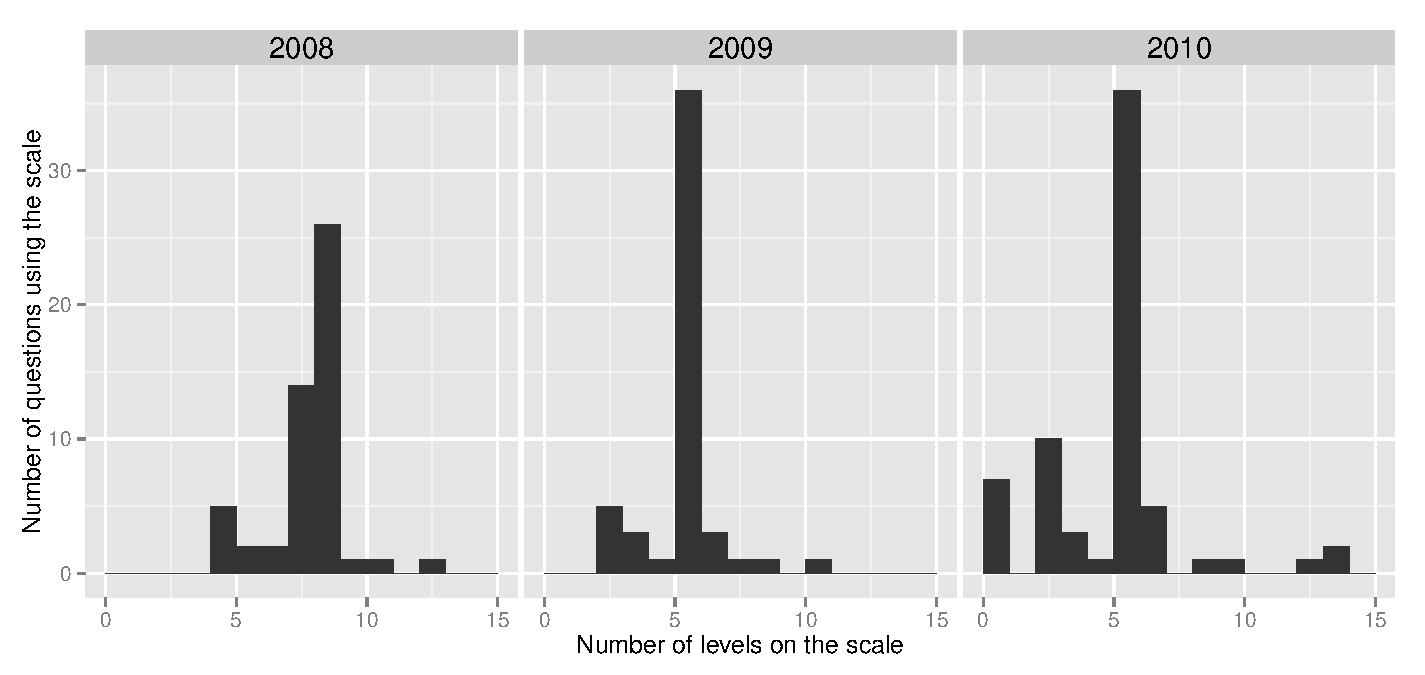
\includegraphics[width=0.99\linewidth]{LikertSizes-1} 

}

\caption[Scale length distributions for each year of the survey]{Scale length distributions for each year of the survey. Notice that the distribution from 2008 is centered around 7, and the 2009 and 2010 distributions are centered around 5. All three distributions have large variation, suggesting that the Knight surveys were quite complex.}\label{fig:LikertSizes}
\end{figure}


\end{knitrout}

\subsection{Missing Data}
\label{missingdata}
While the Gallup reports claim the telephone surveys only took 15 minutes, the number of variables collected and the wide range of response scales seems to indicate a much larger time commitment. This raises the question of whether everyone who began the survey completed it. And, as mentioned in Section \ref{maprates}, the 2010 data contained many more observations than previous years. The explanation for this difference is missing data, presumably related to surveys that were not fully completed. 



In order to explore this, we study the pattern of missing data within the 2010 data set. This data set includes a large number of responses that are extremely sparse, containing almost no completed survey questions, but generally completed demographic information. For example, the question ``How likely are you to recommend this community to a friend or associate as a place to live?'' has 4947 missing values, and the question ``The overall quality of the colleges and universities'' has 5200 missing values. Just between those two questions, the overlap of missing values for both questions is 4887. In other words, almost all the entries that are missing a response to the question about recommending the community are also missing a response to the question about colleges. Similarly, there are 4887 respondents missing both the question about colleges and the question ``Are you registered to vote?''

These questions were chosen arbitrarily, but the pattern is almost the same no matter which pair of survey questions was selected. As a result, we chose to use the question about recommending the community to a friend or associate as a proxy for the overall missing data. That is, if the response was missing an answer to that question, we considered it to be a ``missing'' response. The particular question was selected as an indicator of missing data because it was the first question on the survey (in order of the survey script) to have this scale of missing data. Better methods could have been used, for example setting a cutoff number of missing questions within a single respondent, but this seemed to be fairly accurate for our purposes. 

In order to be consistent, we have considered data missing in 2008 and 2009 if there was no response to the question ``How likely are you to recommend this community to a friend or associate as a place to live?'' even though the 2008 and 2009 data do not show the same correspondence between that question being missing and the rest of the responses being almost completely sparse. Table \ref{missingtable} shows the percentage of data designated as missing for each survey year. While the 2008 and 2009 data sets are almost complete, the 2010 data set has about 25\% missing data.

Interestingly, with the incomplete responses removed, the 2010 data set is reduced to ~15,000 observations, which is much closer to the ~14,000 observations the two prior years. This suggests that incomplete responses were removed in previous years, or that some new survey methodology (i.e. a ``short form'') was introduced in 2010. 

% latex table generated in R 3.1.2 by xtable 1.7-3 package
% Fri Mar 13 16:55:39 2015
\begin{table}[ht]
\centering
\begin{tabular}{rrrr}
  \hline
Year & Missing & Total & Percent \\ 
  \hline
2008 &   6 & 13822 & 0.04 \\ 
  2009 &  63 & 13728 & 0.46 \\ 
  2010 & 4947 & 20271 & 24.40 \\ 
   \hline
\end{tabular}
\caption{Percent of missing data from surveys. The 2010 survey has almost 25 percent missing data. The total number of entries in 2010 is also much larger, suggesting that the 2008 and 2009 datasets used a different criteria for inclusion of entries.} 
\label{missingtable}
\end{table}


\section{Community Satisfaction}
\label{communittsatsec}
Knowing that the question about community satisfaction was the only survey question answered by all respondents, it made sense to see which communities reported the highest levels of community satisfaction. 

To visualize this, a set of stacked distribution graphs were created \citep{RobHei2011}. These stacked distribution graphs are centered around zero and use a diverging color scale to give an overall graphical sense of the amount of positive and negative responses across groups. Figure \ref{fig:communitysatplot} shows the distribution of responses to the question, ``Taking everything into account, how satisfied are you with this community as a place to live?'' and is ordered by the communities with the largest total positive responses in 2008, which highlights the changes in 2009 and 2010. 



\begin{knitrout}
\definecolor{shadecolor}{rgb}{0.969, 0.969, 0.969}\color{fgcolor}\begin{figure}

{\centering 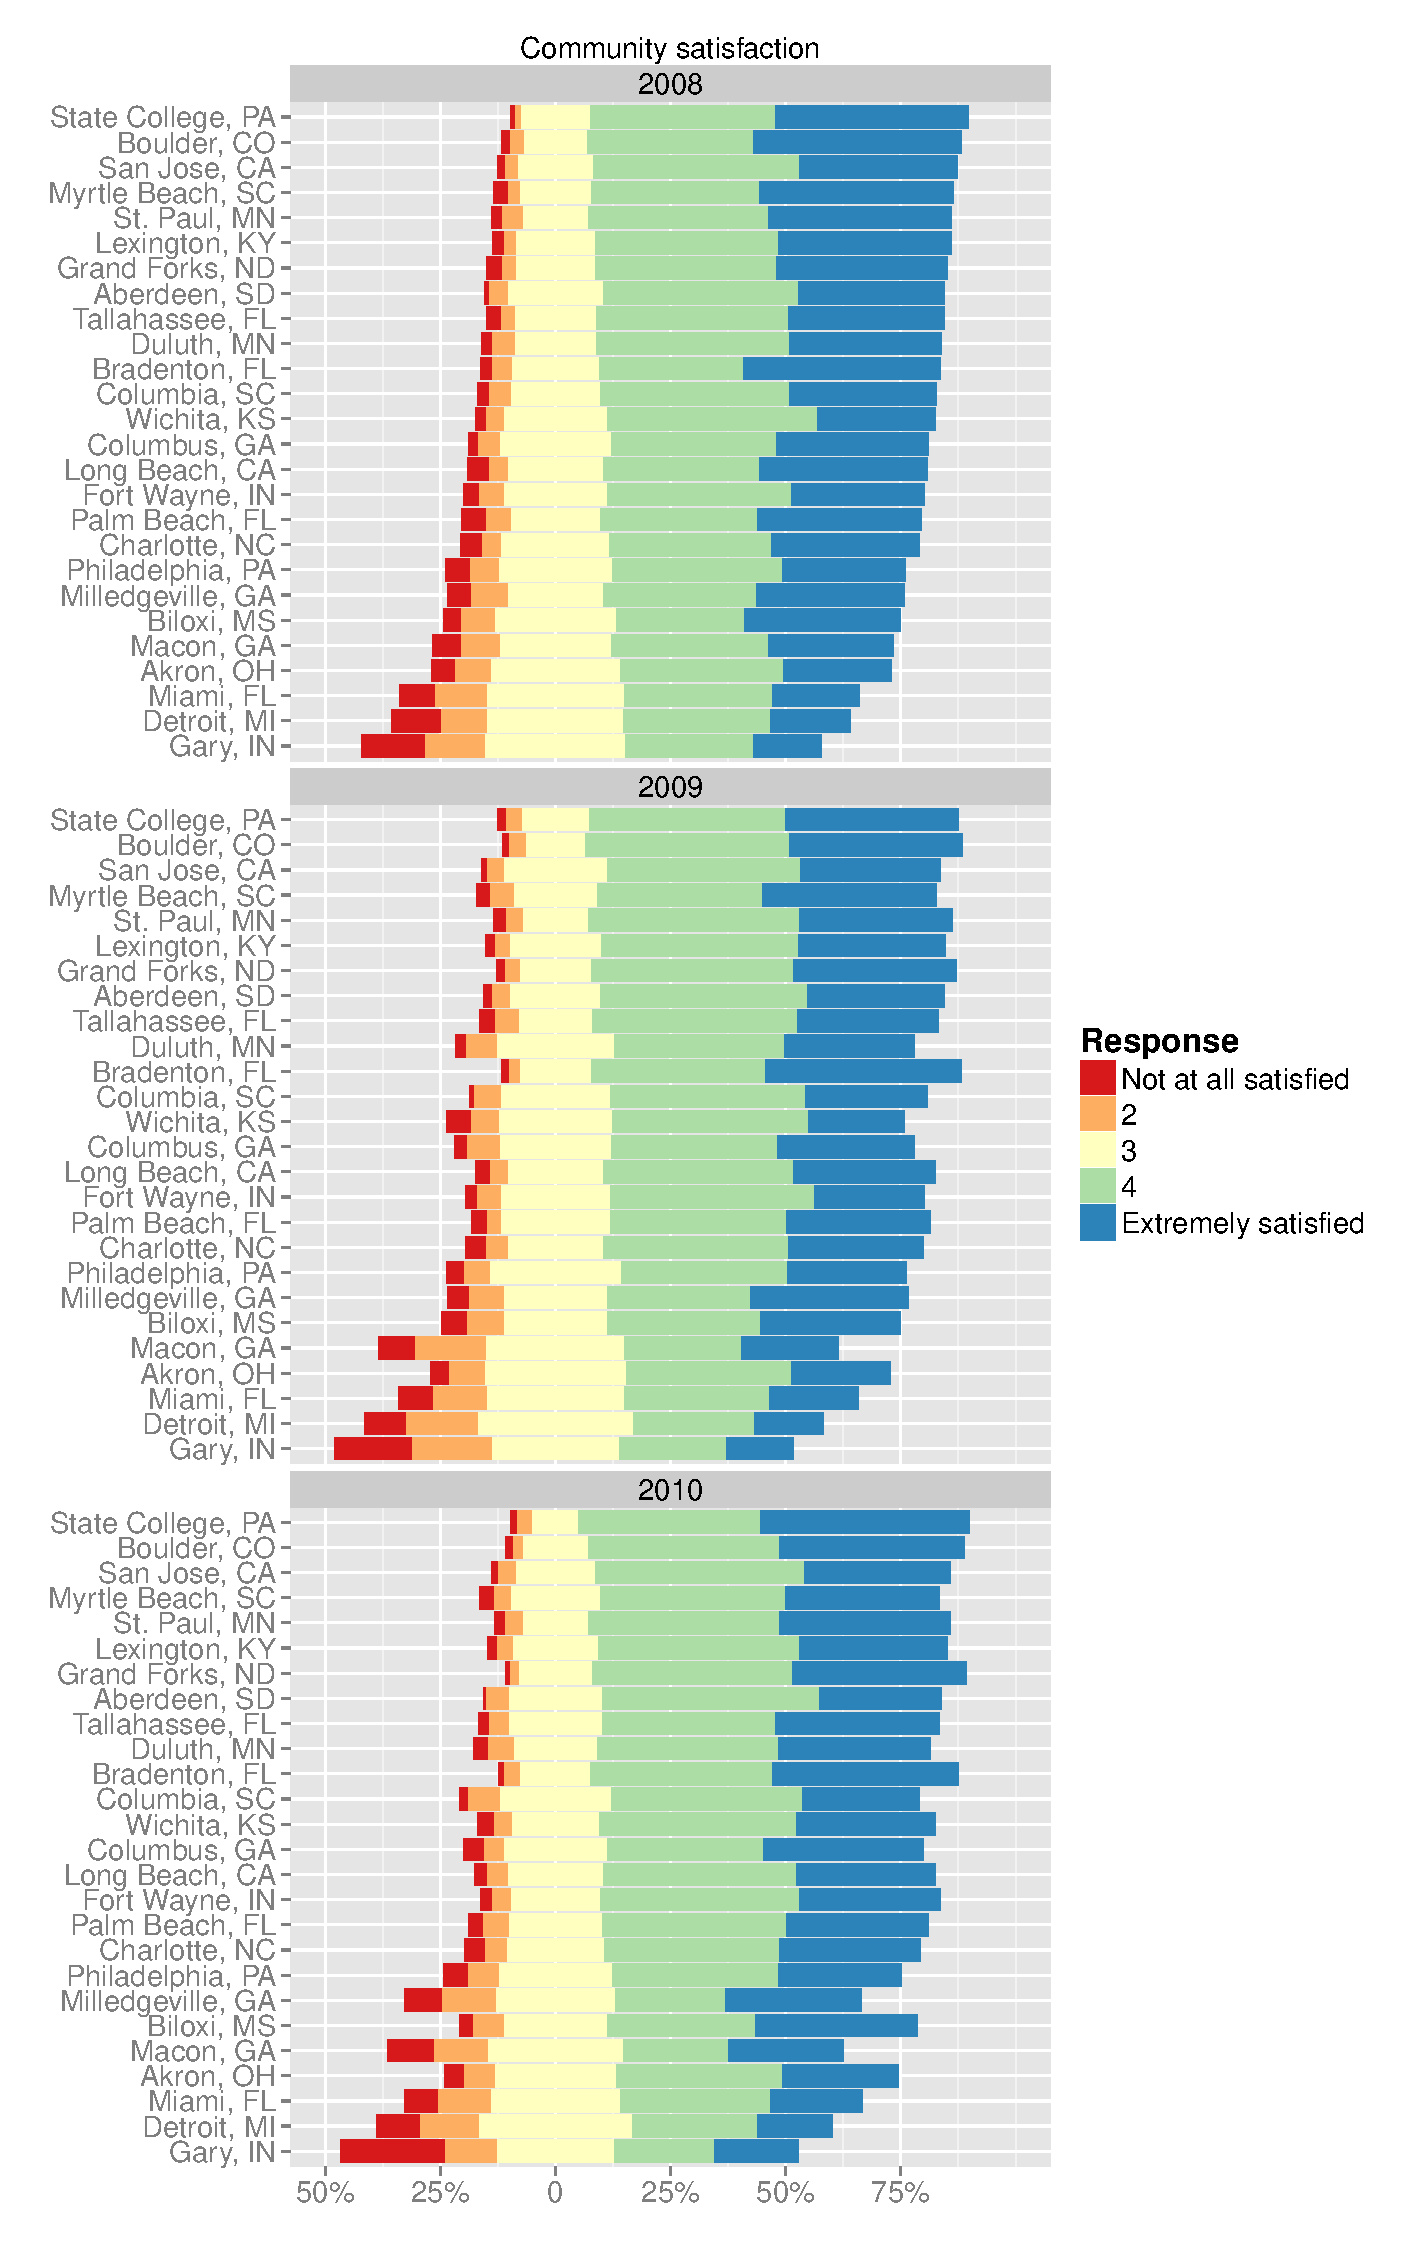
\includegraphics[width=0.99\linewidth]{communitysatplot-1} 

}

\caption[Responses to the question, ``Taking everything into account, how satisified are you with this community as a place to live?" Communities are ordered by percentage of positive responses in 2008, making it clear the differences in distribution in 2009 and 2010]{Responses to the question, ``Taking everything into account, how satisified are you with this community as a place to live?" Communities are ordered by percentage of positive responses in 2008, making it clear the differences in distribution in 2009 and 2010.}\label{fig:communitysatplot}
\end{figure}


\end{knitrout}

Overall, the total percentage of positive responses in 2008 ranges between 58\% on the low end, and 90\% at the high end. These numbers are the overall percentage of people in each community that are answering the question, ``Taking everything into account, how satisfied are you with this community as a place to live?'' positively (this includes half of the responses labeled 3).

Communities are ordered by overall positive responses in 2008, which allows for comparisons between communities and across years. The overall trend is fairly stable, but there is some variation, both positive and negative. Looking at Figure \ref{fig:communitysatplot}, we can see that people in State College, PA typically report much greater levels of community satisfaction than people in Detroit, MI or Gary, IN. After 2008, Macon, GA sees a decrease in overall community satisfaction, moving from 73\% in 2008 to 61\% in 2009 and slightly up to 63\% in 2010. Over the same time period, Bradenton, FL shows a slight increase in community satisfaction, from 84\% in 2008 to about  88\% in 2009 and 2010. 

\section{Community Engagement through Local Behaviors}
\label{behaviorsec}
Another point of interest was the most common behaviors reported by participants. Figure \ref{fig:YNall} shows the percentage of participants engaging in a variety of behaviors over the three years of the survey. An additional set of questions were introduced in 2010, so those are necessarily blank in the previous years. 

Behaviors are arranged by percentage of survey respondents who reported the behavior. 
Over all three years, the most common behavior was being registered to vote, followed by voting in a local election. The least common responses to the behavior questions (considering all three years) were ``worked with other residents to make change in the local community'', and ``attended a local public meeting in which local issues were discussed.'' When the additional questions were added in 2010, an even-less-common behavior was added, ``gave money or food to an individual in need in your community who is not related to you.'' 



\begin{knitrout}
\definecolor{shadecolor}{rgb}{0.969, 0.969, 0.969}\color{fgcolor}\begin{figure}

{\centering 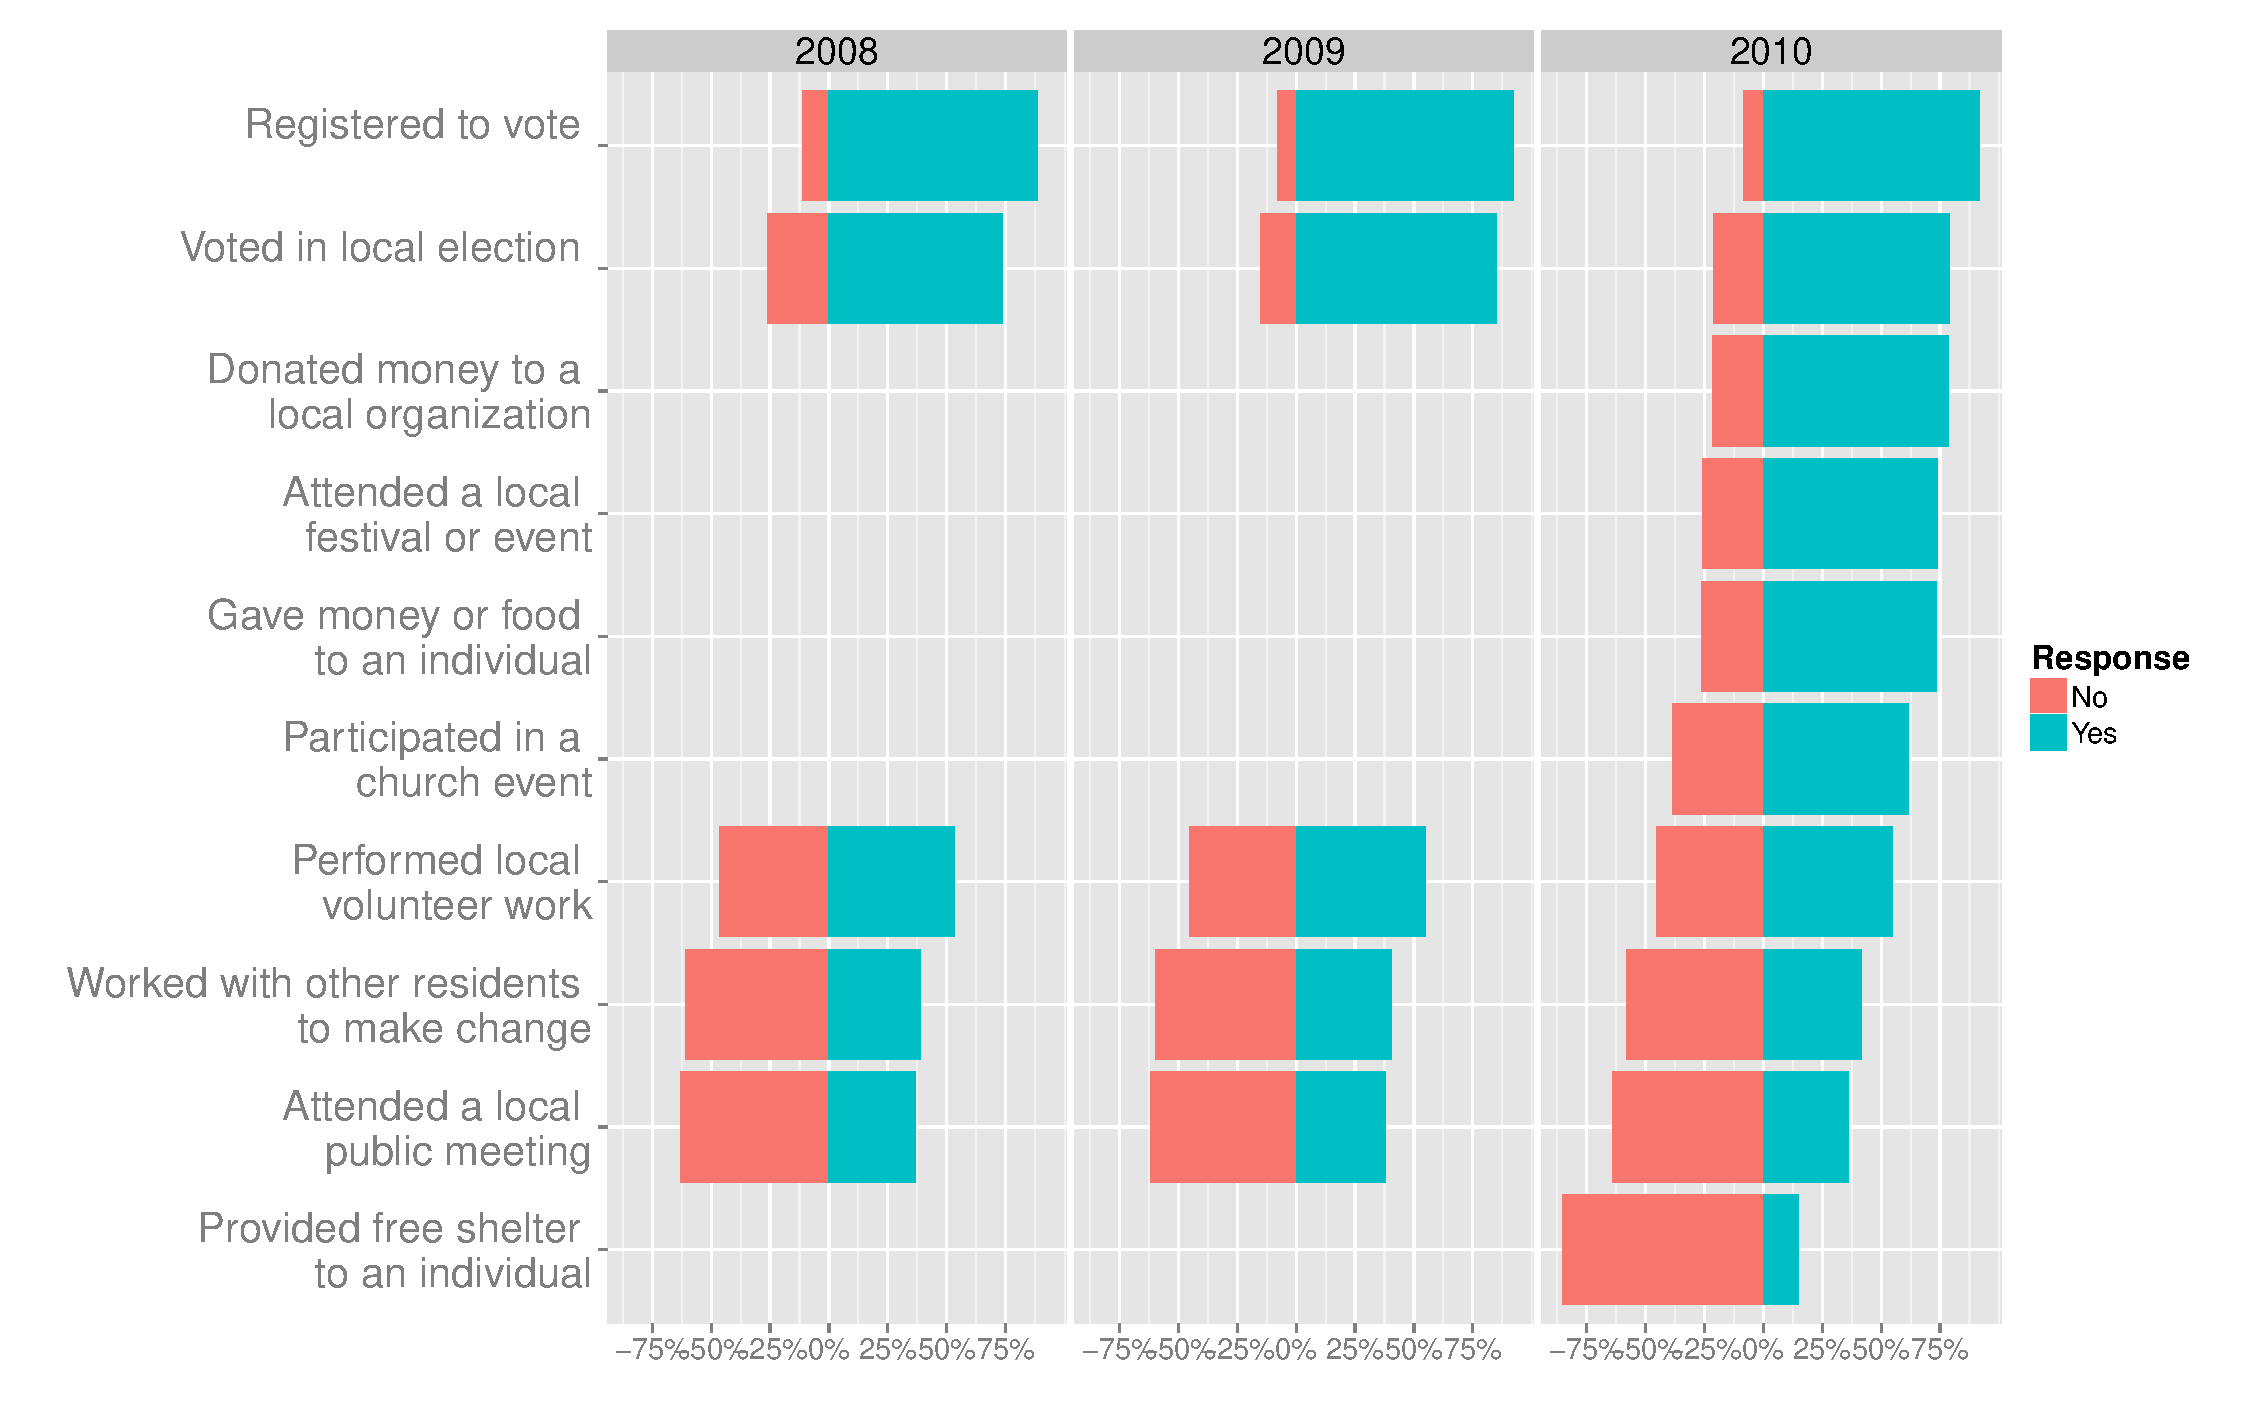
\includegraphics[width=0.99\linewidth]{YNall-1} 

}

\caption[Responses to yes/no questions about participants' behaviors, comparing all three survey years]{Responses to yes/no questions about participants' behaviors, comparing all three survey years.}\label{fig:YNall}
\end{figure}


\end{knitrout}





\begin{knitrout}
\definecolor{shadecolor}{rgb}{0.969, 0.969, 0.969}\color{fgcolor}\begin{figure}

{\centering 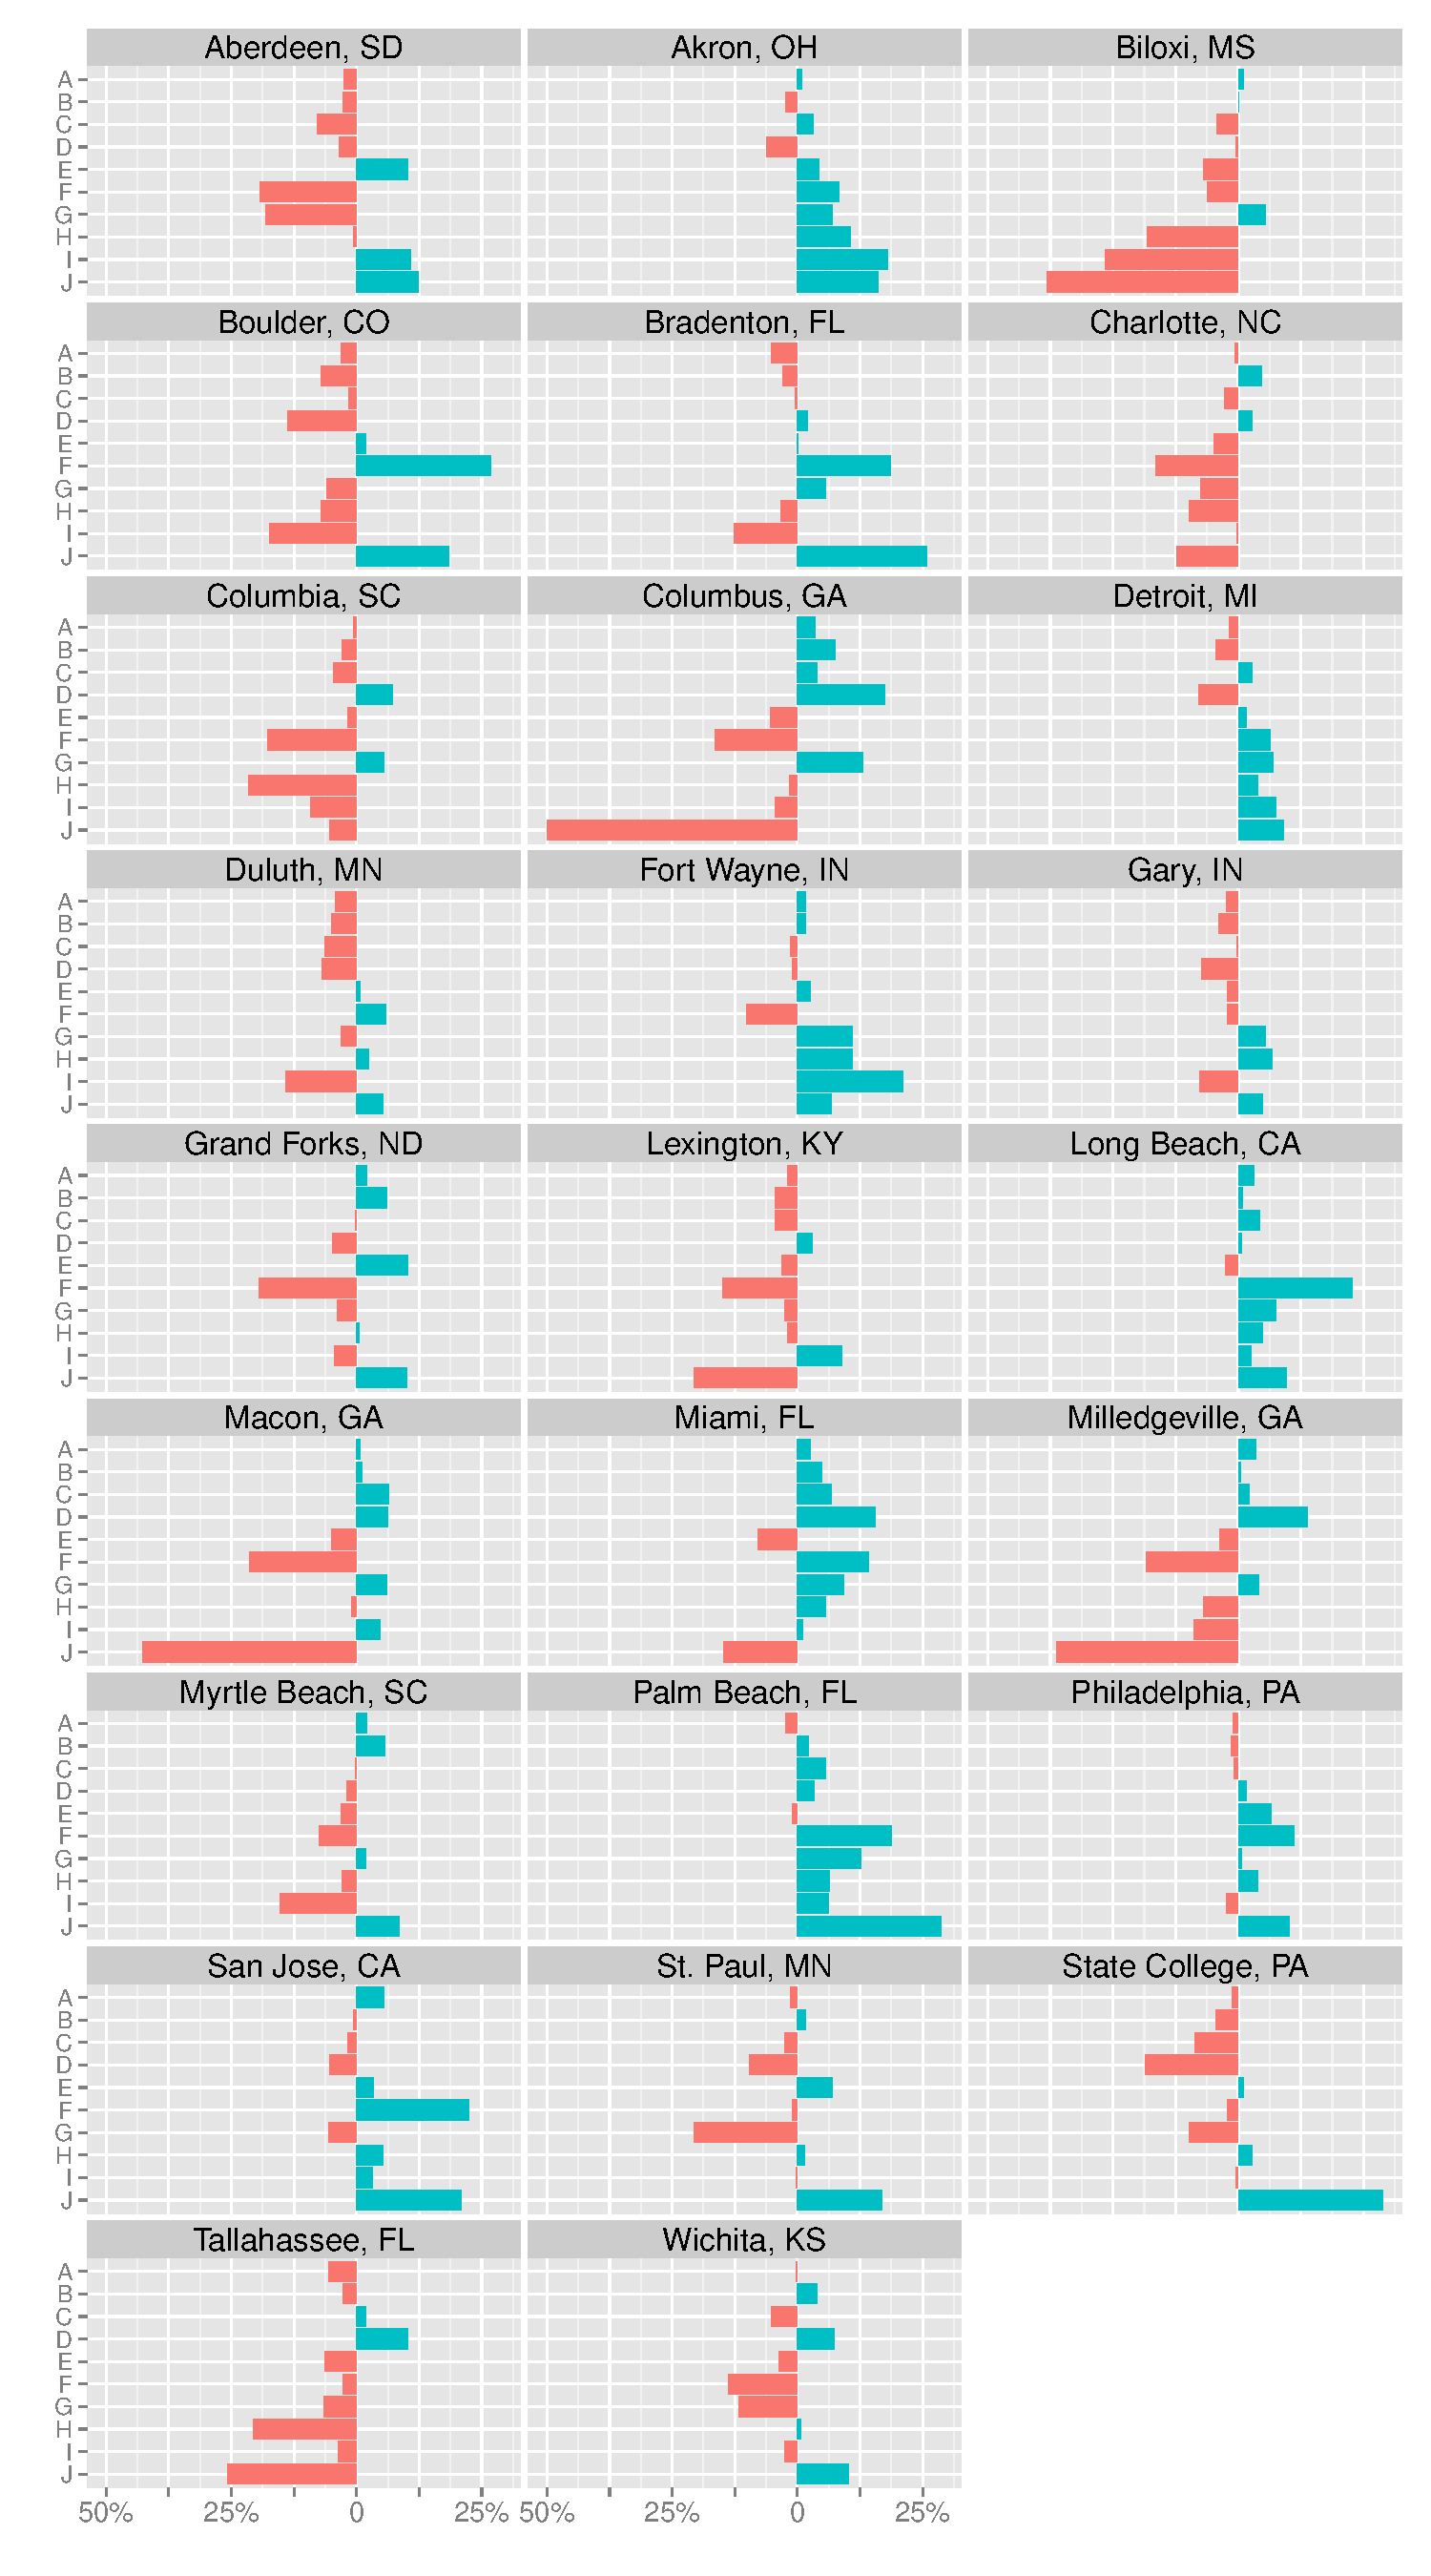
\includegraphics[width=0.99\linewidth]{YN2010plot-1} 

}

\caption{Percentage difference from overall survey rates (2010 data). The letters A-J represent the activities listed in Figure \ref{fig:YNall}. A: Registered to vote, B: Voted in a local election, C: Donated money to a local organization, D: Attended a local event, E: Gave money or food to an individual, F: Participated in a church event, G: Performed local volunteer work, H: Worked with other residents to make change, I: Attended a local public meeting, J: Provided free shelter to an individual.}\label{fig:YN2010plot}
\end{figure}


\end{knitrout}

A followup to this question is whether all communities performed these actions at similar rates, or if there were local variations in behavior. Figure \ref{fig:YN2010plot} shows the difference from the overall rate across all 26 communities and 10 behaviors in 2010. More study is required to determine if the visual differences between communities represent true differences or just random variation, but there are certainly communities that stand out from the rest. 

For example, people in St. Paul, MN, San Jose, CA, and State College, PA were much more likely than the average to to provide free shelter to a non-relative, while people in Georgia (both Macon and Milledgeville) were less likely to. This provides a connection to Figure \ref{fig:communitysatplot}, because Macon and Milledgeville were the two communities whose community satisfaction scores decreased the most in 2009 and 2010, while San Jose was one of the most satisfied communities over all three years. One hypothesis is that St. Paul, San Jose, and State College are all university towns, where young people (especially college students) may invite friends and friends-of-friends to stay with them for free. Again, more study is required. 

It is also interesting to note the communities that performed above or below national rates on most questions. For example, Biloxi, MS shows that respondents are much less likely to engage in any of the behaviors asked about, with the exception of being registered to vote and performing local volunteer work. On the other hand, Palm Beach, FL shows higher-than-average rates for almost all behavior, except for being registered to vote and giving money or food to an individual. Long Beach, CA shows a similar pattern. However, since this array of plots represents 26 facets of the same plot, it is possible that these visual trends occurred by chance. 

\section{Meta-Knowledge}
\label{metasec}
The primary aim  of this article is to address whether communities hold meta-knowledge about their city being a good place for subgroups or minorities. 

The survey asks a number of questions related to rating the community as a place for subgroups, including: ``young, talented college graduates,'' ``immigrants from other countries,'' ``racial and ethnic minorities,'' ``families with young children,'' ``gay and lesbian people,'' ``senior citizens,'' and ``young adults without children.'' Not all these subgroups were asked to identify themselves in the demographic questions (particularly ``gay and lesbian people'') so it was not possible to address them all. Instead, we focus on racial and ethnic minorities, senior citizens, and families with young children.

Community meta-knowledge is essentially majority group empathy or understanding of how minorities experience their community. For example, the survey asks participants to rate their community as a place for families with young children on a 5-point Likert scale. A city where participants with children rated their community in the same way as participants without children is defined as a community with high meta-knowledge about conditions for families with young children. 

Ideally, we could use the information gathered about community meta-knowledge on subgroup experiences to determine more about the community itself. It's possible that meta-knowledge would correlate with other measures we are interested in (for example, overall community satisfaction). 

We define meta-knowledge for a particular dimension (e.g. seniors) as the difference between the total percentage of positive responses to the question, ``How is your community as a place for [particular subgroup]?" by people in the subgroup and those outside it. This can be expressed by equation (\ref{MK}). 

\begin{eqnarray}
\label{MK}
MK = \sum R^{+}_{\mbox{ In subgroup}} - \sum R^{+}_{\mbox{ Out of subgroup}}
\end{eqnarray}

We can calculate $MK$ for each subgroup we are interested in, denoting which group we are talking about by a subscript. Here, we will consider the questions ``How is your community as a place for racial and ethnic minorities?'' ($MK_R$), ``How is your community as a place for seniors?'' ($MK_S$), and ``How if your community as a place for families with young children?'' ($MK_C$).

Using this definition, communities where Whites highly over-rate their community as a place for minorities will have a negative $MK_S$ score, while communities where Whites under-rate their community will have a positive $MK_S$ score. Communities where the ratings by both groups are roughly equal have a $MK_S$ score of zero. 

For a visual explanation of this rating system, see Figure \ref{fig:anotherlookplot}. Points above the $y=x$ line will have a negative $MK$ score, those below the line will have a positive score, and those on the line will be zero.

This definition puts emphasis on communities where out-of-subgroup participants rated their city the same way that in-subgroup participants did, based on the assumption that empathy is important to communities \citep{SteFin1999}. 

\subsection{Meta-knowledge about the community as a place for racial and ethnic minorities}
\label{minorities}
To begin, we investigate meta-knowledge about racial and ethnic minorities. This proved somewhat difficult because each year of data collection used a slightly different set of possible answer choices to the question ``Which of these groups best describes your racial background?'' and because there were so many participants who refused to answer (particularly in 2010). 



\begin{knitrout}
\definecolor{shadecolor}{rgb}{0.969, 0.969, 0.969}\color{fgcolor}\begin{figure}

{\centering 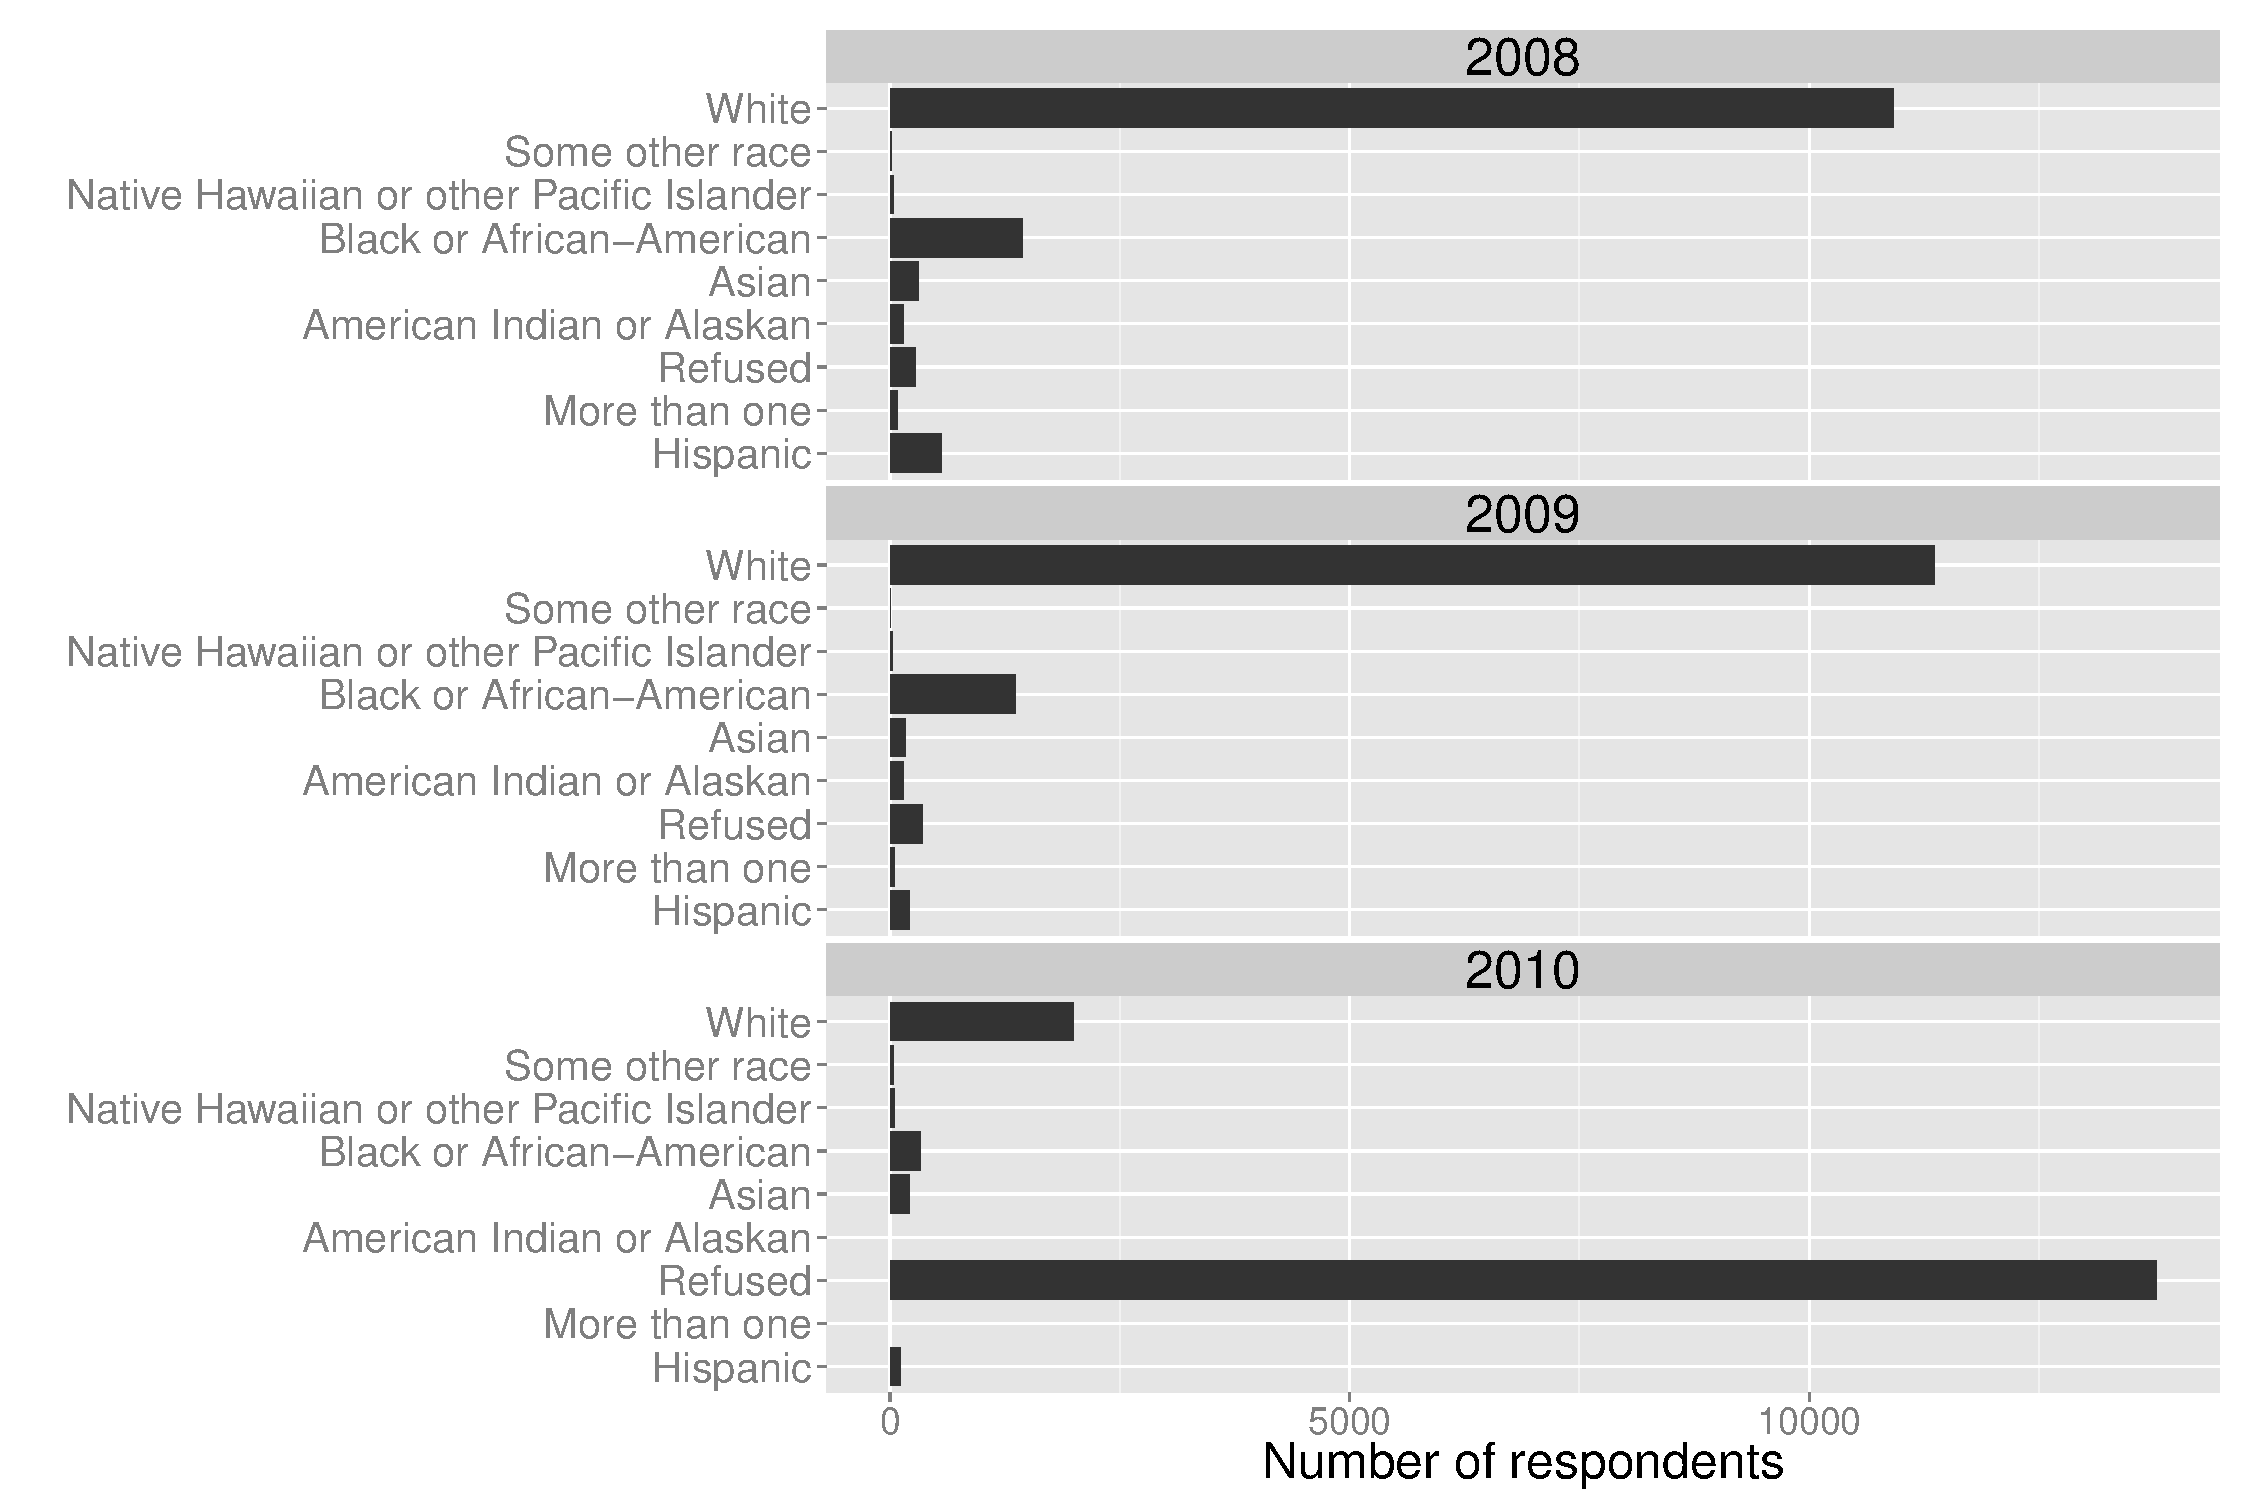
\includegraphics[width=0.99\linewidth]{overallRaceplot-1} 

}

\caption[Responses to the question, ``Which of these groups best describes your racial background?" Notice that 2010 shows an overrepresentation of Refused responses, compared to the other years]{Responses to the question, ``Which of these groups best describes your racial background?" Notice that 2010 shows an overrepresentation of Refused responses, compared to the other years.}\label{fig:overallRaceplot}
\end{figure}


\end{knitrout}

The overall distribution of responses to the demographic race question is shown in Figure \ref{fig:overallRaceplot}. This figure is shown with absolute numbers of participants, rather than fractions, to underscore how different the 2010 data is. Notice that in 2010, the largest category was ``Refused,'' and without that category the rest of the responses are not on the same scale as previous years. As the plot shows, the sample sizes for individual minority race responses were somewhat small each year, so for the investigation on subgroup meta-knowledge, we combined all the minority responses into one group that we refer to as Non-white. This category contains all participants who reported a race that was not White, but does not include participants who declined to give a response to the question. For a condensed summary of what the White/Non-white criteria means for the overall percentages, see Figure \ref{fig:samplesize}. 



\begin{knitrout}
\definecolor{shadecolor}{rgb}{0.969, 0.969, 0.969}\color{fgcolor}\begin{figure}

{\centering 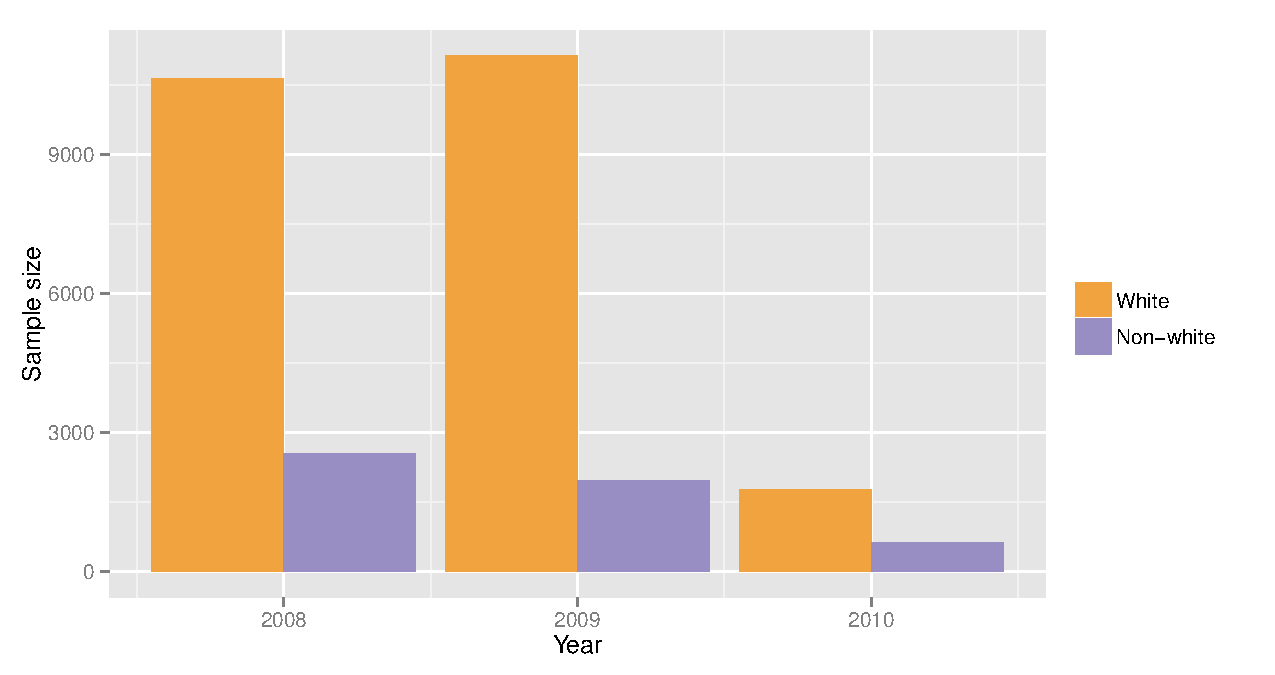
\includegraphics[width=0.99\linewidth]{samplesize-1} 

}

\caption[Sample sizes for plots about meta-knowledge regarding the community as a place for minorities]{Sample sizes for plots about meta-knowledge regarding the community as a place for minorities.}\label{fig:samplesize}
\end{figure}


\end{knitrout}

\begin{knitrout}
\definecolor{shadecolor}{rgb}{0.969, 0.969, 0.969}\color{fgcolor}\begin{figure}

{\centering 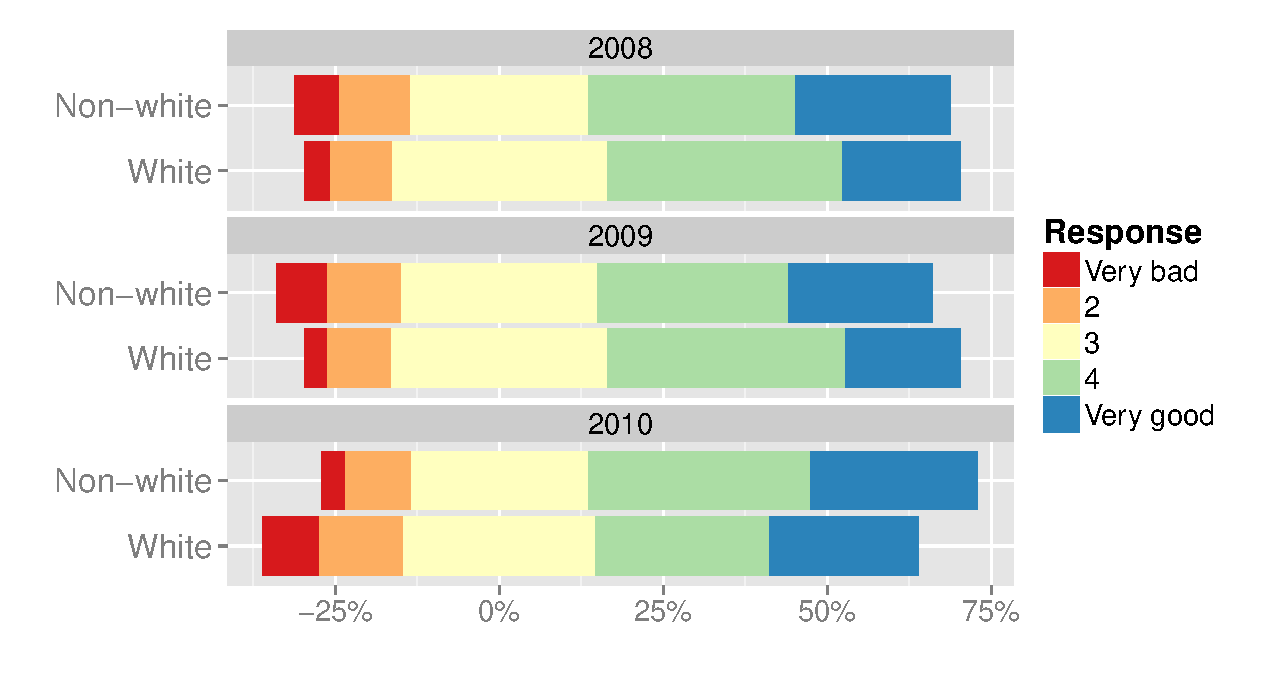
\includegraphics[width=0.99\linewidth]{overallRaceResponsePlot-1} 

}

\caption{Responses to the question, ``How is your community as a place for racial and ethnic minorities?" White denotes survey respondents who listed their race as White, and Non-white is all other race responses (not including survey participants who refused to report a race). Notice the difference between the 2008/2009 responses and the 2010 responses, but also refer to Figure \ref{fig:samplesize} for the absolute sample sizes for each year-- 2010 has a much smaller sample of responses to the question overall.}\label{fig:overallRaceResponsePlot}
\end{figure}


\end{knitrout}





\begin{knitrout}
\definecolor{shadecolor}{rgb}{0.969, 0.969, 0.969}\color{fgcolor}\begin{figure}

{\centering 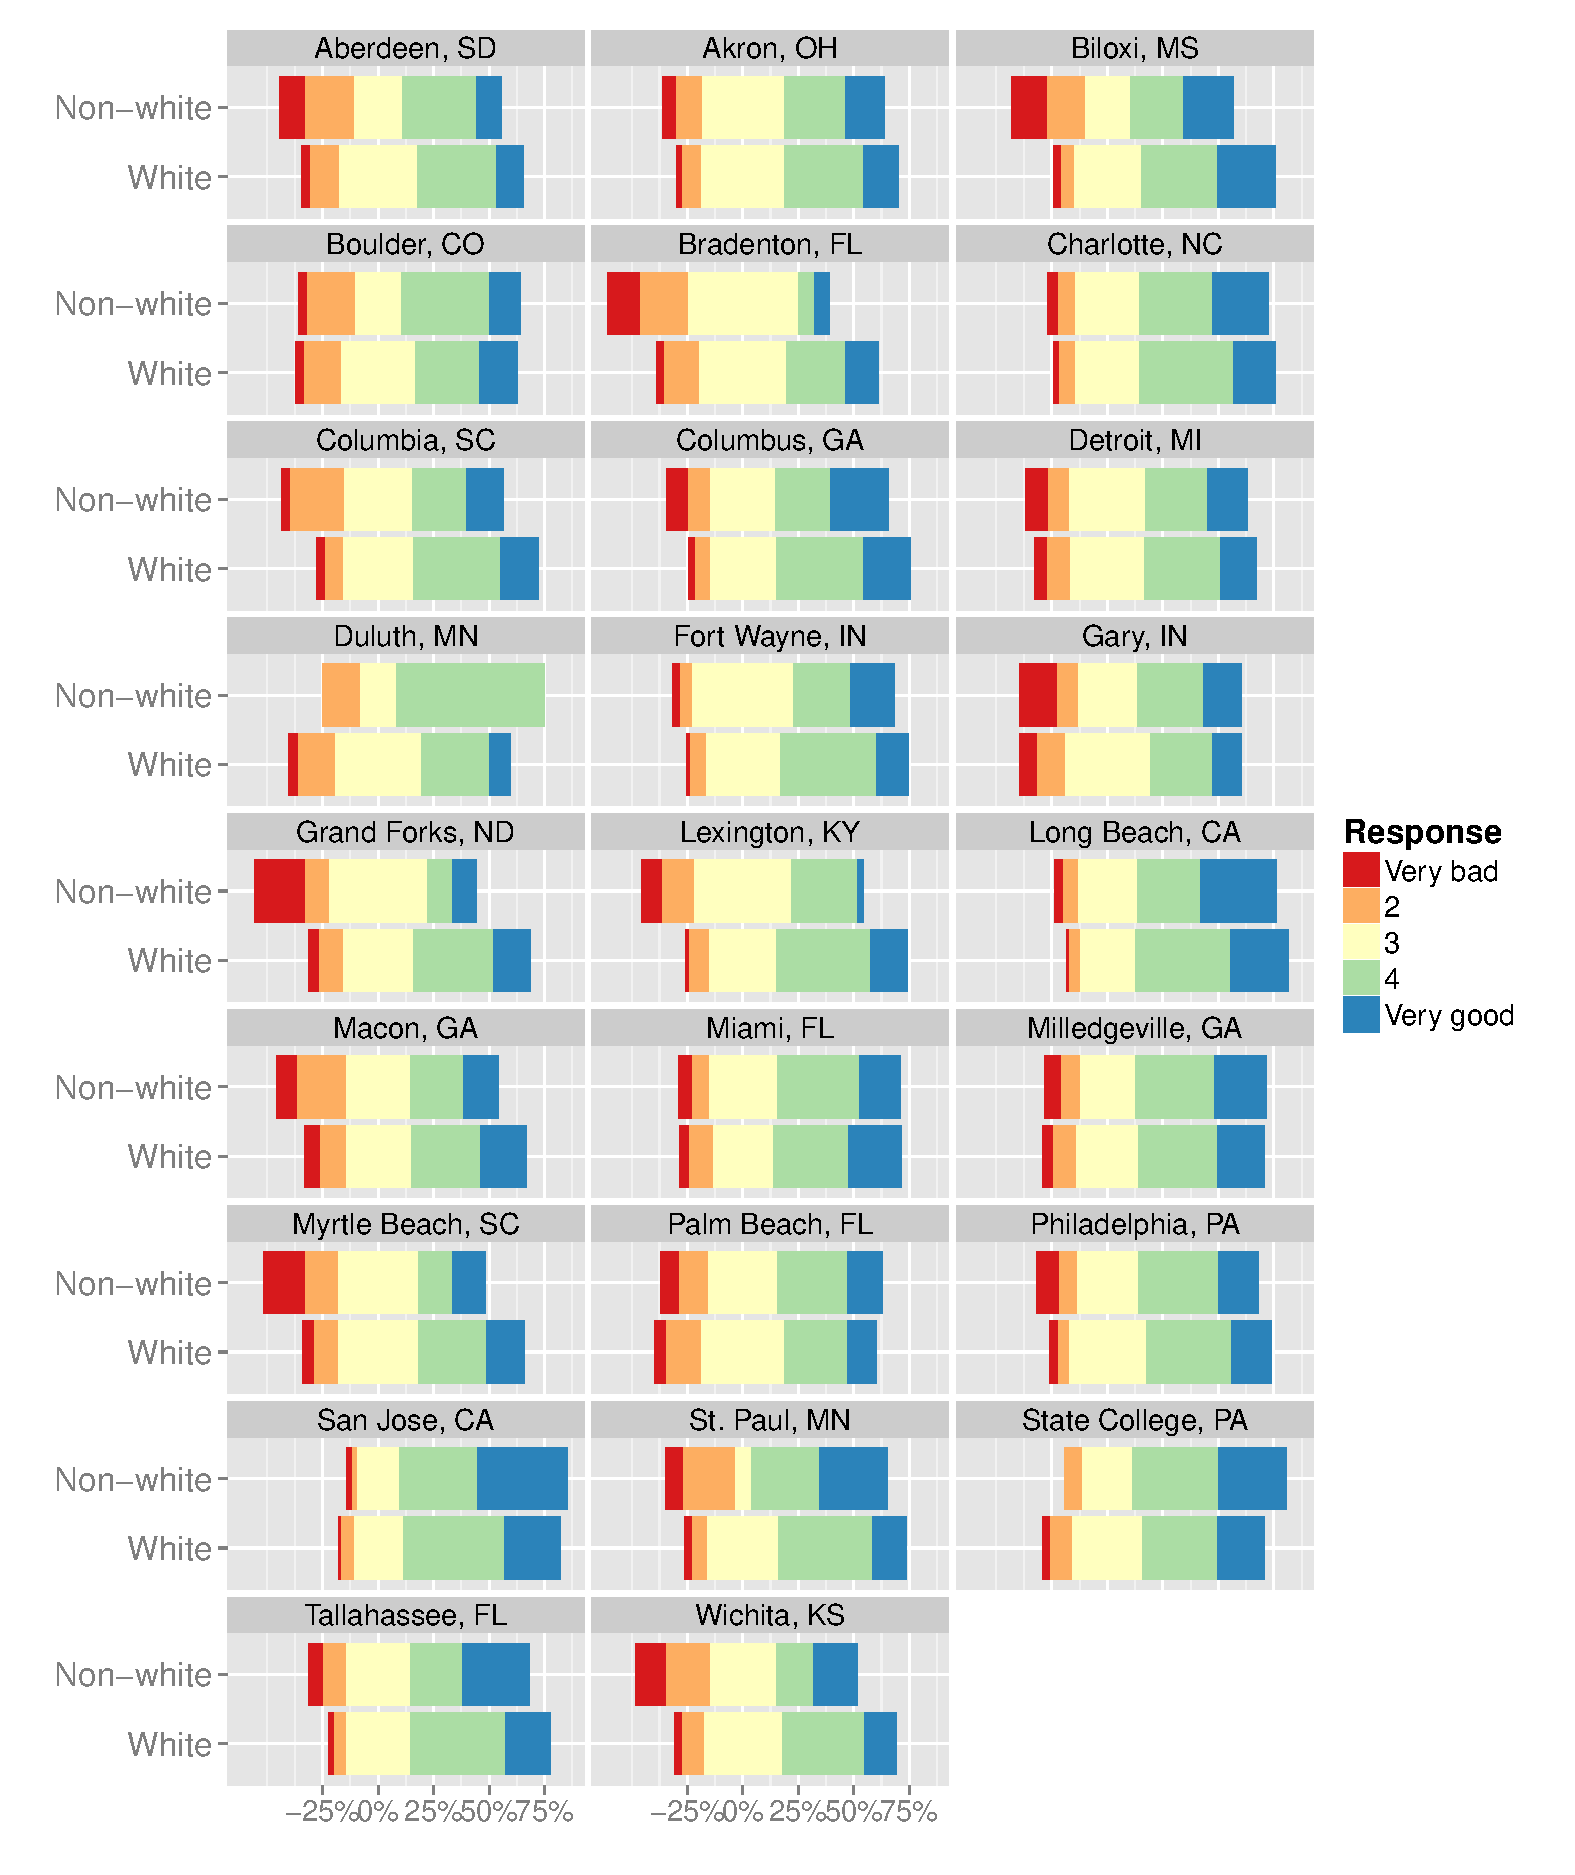
\includegraphics[width=0.99\linewidth]{allMinorities-1} 

}

\caption[Responses to the question, ``How is your community as a place for racial and ethnic minorities?" faceted by community (2009 data)]{Responses to the question, ``How is your community as a place for racial and ethnic minorities?" faceted by community (2009 data).}\label{fig:allMinorities}
\end{figure}


\end{knitrout}

We want to study the overall difference between in-group and out-group responses to the question, ``how is your community as a place for racial and ethnic minorities?'' To do this, the data is split into two groups, one called White and one called Non-white. For comparison of the distribution of responses between groups, see Figure \ref{fig:overallRaceResponsePlot}. Interestingly, Whites were rating their communities as better places for minorities than Non-whites in 2008 and 2009, but in 2010 Whites began under-rating their communities. 

As in Section \ref{behaviorsec}, we want to see the individual variation between communities. We chose to look at the 2009 data to study community-level variation. The community-level responses are shown in Figure \ref{fig:allMinorities}. There is a lot of variation between the communities for this particular type of meta-knowledge. Some communities saw the White respondents over-scoring their community as a place for minorities, while some were under-scoring. 

For the most part, however, Whites over-rated their communities as a place for racial and ethnic minorities, compared to Non-whites. Grand Forks, ND, was a particularly bad offender-- Whites over-rated it as a place for minorities, and minorities themselves rated it as one of the worst communities in 2009. 

There was a lot of additional variation in response distribution. For example, San Jose, CA is highly rated as a place for minorities both by people in- and -outside the subgroup. And it was slightly under-rated by Whites, which is probably a good sign of meta-knowledge and empathy. Going the opposite direction are Grand Forks, ND, Myrtle Beach, SC, and Macon, GA. 

For another view of the relationship between ratings (as seen in Figure \ref{fig:allMinorities}) see Figure \ref{fig:anotherlookplot}, which shows the relationship between  total positive responses by Whites versus total positive responses by Non-whites to the question, ``How is your community as a place for racial and ethnic minorities?'' Figure \ref{fig:anotherlookplot} makes it clear that there are communities that are under- and over-rated by Whites, and those that are closer to the 1-1 (or y=x) line. 

However, even if a community is on the 1-1 line, it may fall below the mean rating for communities overall. Gary, IN is a good example. While it is rated almost exactly the same by Whites and Non-whites, those ratings fall substantially below the mean ratings of communities overall. So, there is agreement that Gary is not a good place for minorities. 



\begin{knitrout}
\definecolor{shadecolor}{rgb}{0.969, 0.969, 0.969}\color{fgcolor}\begin{figure}

{\centering 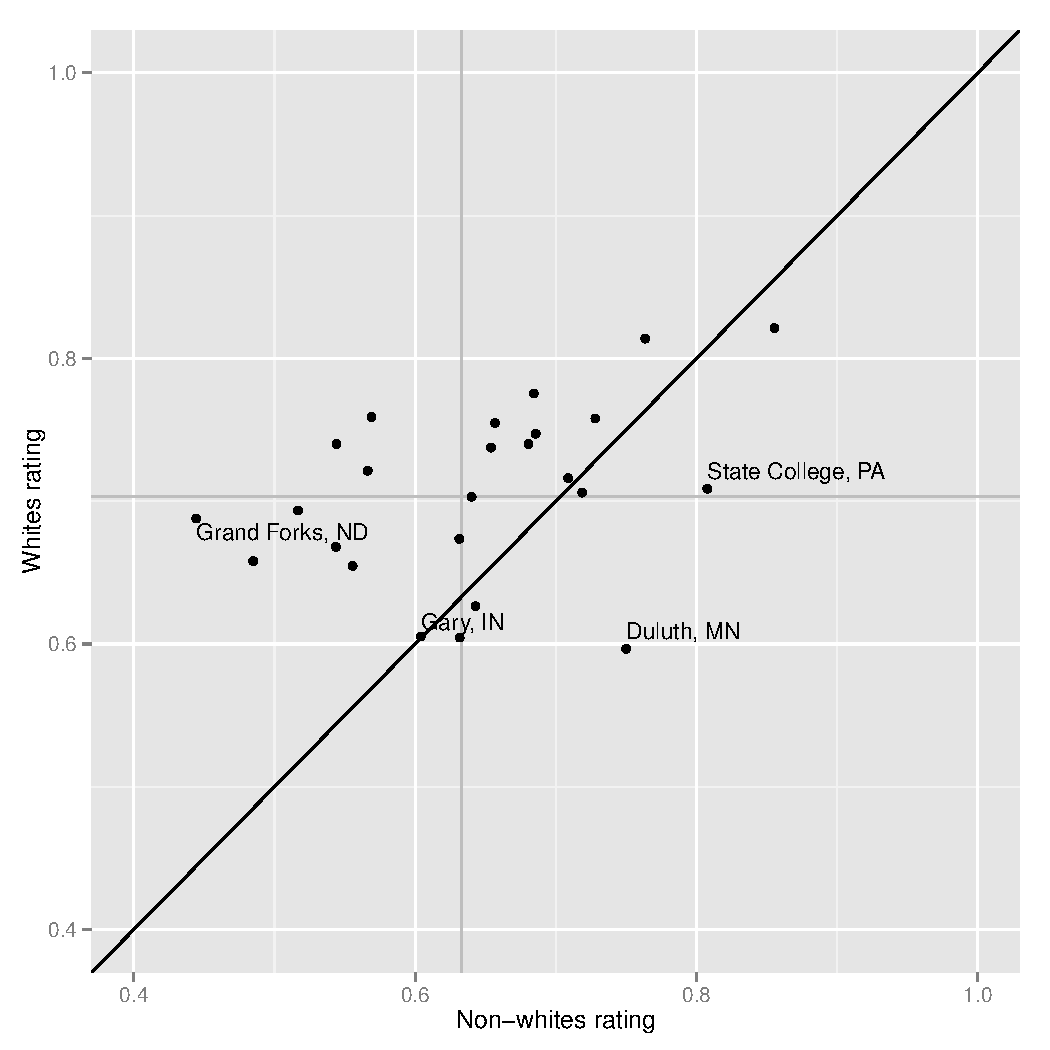
\includegraphics[width=0.76\linewidth]{anotherlookplot-1} 

}

\caption[Relationship between positive responses to the question, ``How is your community as a place for minorities?" comparing ratings of Whites and Non-whites]{Relationship between positive responses to the question, ``How is your community as a place for minorities?" comparing ratings of Whites and Non-whites. Each community is represented, and the plot uses 2009 data. Some communities, like State College, PA, are under-rated by Whites, some are over-rated, like Grand Forks, ND, and some are rated the same by both groups, like Gary, IN. The black line shows y=x, for comparison. Grey lines at x=0.63 and y=0.7 show the mean ratings by each group.}\label{fig:anotherlookplot}
\end{figure}


\end{knitrout}

There is clearly some relationship between ratings by Whites and Non-whites, although it is not a perfect $y=x$ relationship. The correlation between ratings is $r= $0.46.



To explore the effect of $MK_R$ on community satisfaction, we plotted raw $MK_R$ score against community satisfaction (from Section \ref{communittsatsec}) and did not find a trend. Instead, it seemed like high $MK_R$ scores, both positive and negative, were associated with higher community satisfaction. So, we calculated the correlation between the absolute value of meta-knowledge score, $|MK_R|$, and community satisfaction, which is 0.3. This includes data from both 2008 and 2009 (2010 data was still excluded because of sample size issues). 

The correlation suggests a positive relationship between the variables, but it's not what we would expect. Communities that had the highest absolute difference in scoring of the question ``how is your community as a place for minorities?'' between Whites and Non-whites (and therefore the highest $|MK_R|$ score) had the highest community satisfaction scores. Communities that had low meta-knowledge score (like Gary, IN) have low community satisfaction scores. This seems counter-intuitive, as we would expect communities that had more self awareness to be more satisfied, but that's not what we see in the plot. It is clear that there is more to community satisfaction than just $|MK_R|$. 


\subsection{Meta-knowledge about the community as a place for seniors}
\label{mseniors}



\begin{knitrout}
\definecolor{shadecolor}{rgb}{0.969, 0.969, 0.969}\color{fgcolor}\begin{figure}

{\centering 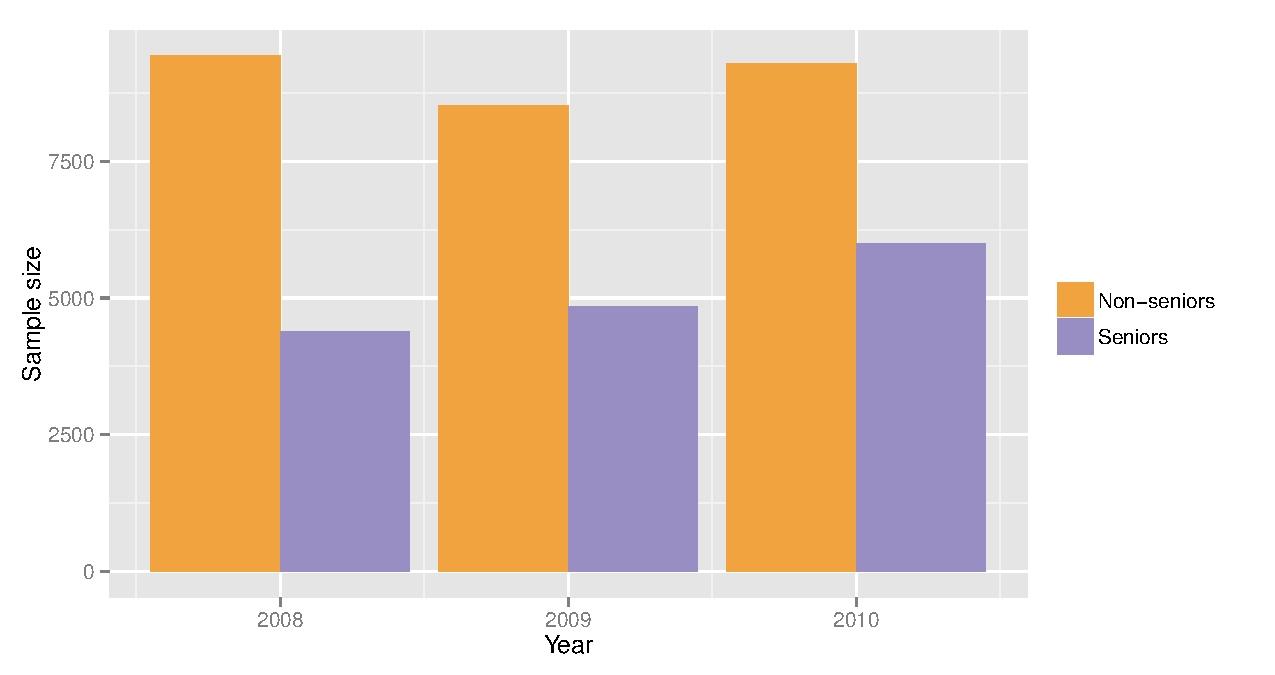
\includegraphics[width=0.99\linewidth]{seniorSS-1} 

}

\caption[Sample sizes for plots about meta-knowledge regarding the community as a place for seniors]{Sample sizes for plots about meta-knowledge regarding the community as a place for seniors.}\label{fig:seniorSS}
\end{figure}


\end{knitrout}




To continue our exploration of meta-knowledge, we consider meta-knowledge about communities as a place for seniors, or $MK_S$. In order to determine if non-seniors understood how good their community was for seniors, the data was split into two pieces, one of participants aged 62 and older, and the other of participants under 62. For sample sizes of the groups, see Figure \ref{fig:seniorSS}.

The yearly ratings distributions are shown in Figure \ref{fig:seniorOverallPlot}. It appears that non-seniors typically underestimate how good a place is for seniors. People 62 and older rated their community as a better place for seniors than did people under 62, over all three years.  

\begin{knitrout}
\definecolor{shadecolor}{rgb}{0.969, 0.969, 0.969}\color{fgcolor}\begin{figure}

{\centering 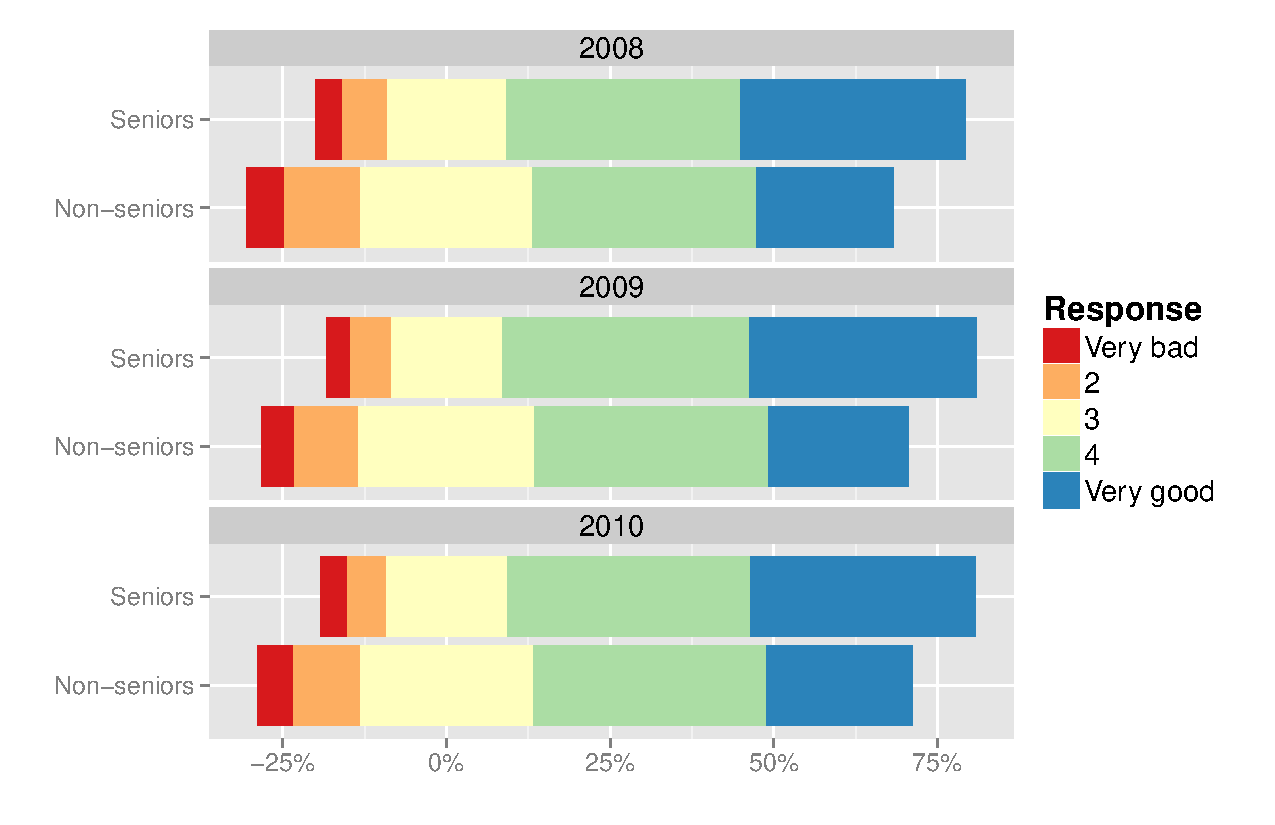
\includegraphics[width=0.99\linewidth]{seniorOverallPlot-1} 

}

\caption[Responses to the question, ``How is your community as a place for seniors?" Seniors are defined as survey participants aged 62 and older, non-seniors are those under 62]{Responses to the question, ``How is your community as a place for seniors?" Seniors are defined as survey participants aged 62 and older, non-seniors are those under 62. Notice that seniors consistently rated their community more highly than did non-seniors over all three survey years.}\label{fig:seniorOverallPlot}
\end{figure}


\end{knitrout}

\begin{knitrout}
\definecolor{shadecolor}{rgb}{0.969, 0.969, 0.969}\color{fgcolor}\begin{figure}

{\centering 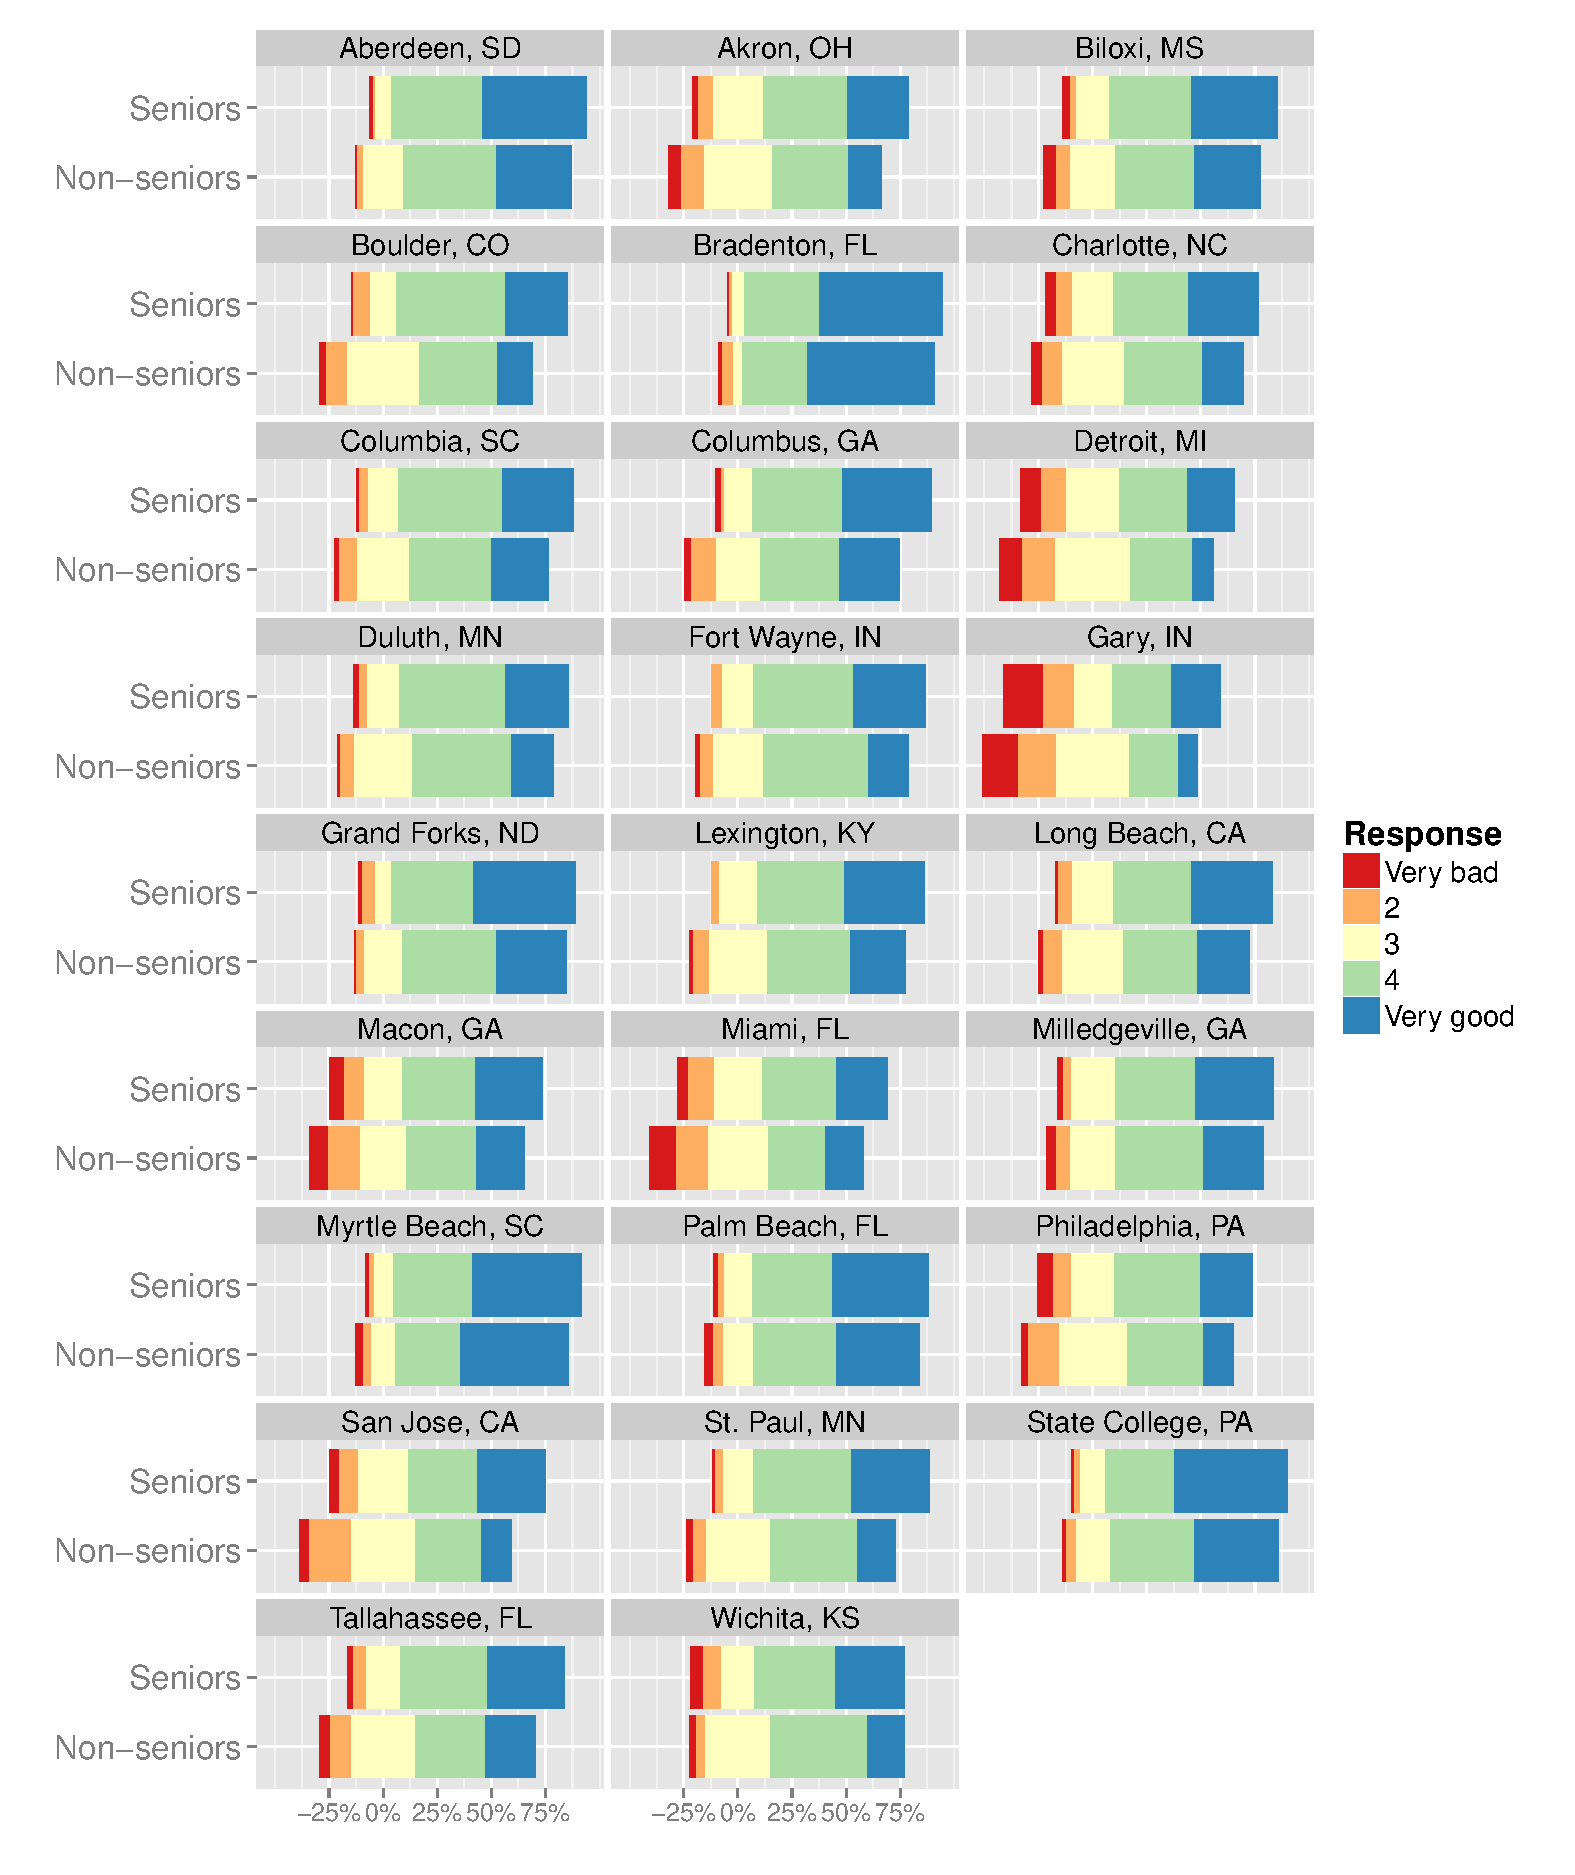
\includegraphics[width=0.99\linewidth]{seniorPlot-1} 

}

\caption[Responses to the question, ``How is your community as a place for seniors?" faceted by community (2009 data)]{Responses to the question, ``How is your community as a place for seniors?" faceted by community (2009 data). Every community follows the pattern of over-rating by seniors, but some communities have a smaller discrepancy between ratings of seniors and non-seniors.}\label{fig:seniorPlot}
\end{figure}


\end{knitrout}


\begin{knitrout}
\definecolor{shadecolor}{rgb}{0.969, 0.969, 0.969}\color{fgcolor}\begin{figure}

{\centering 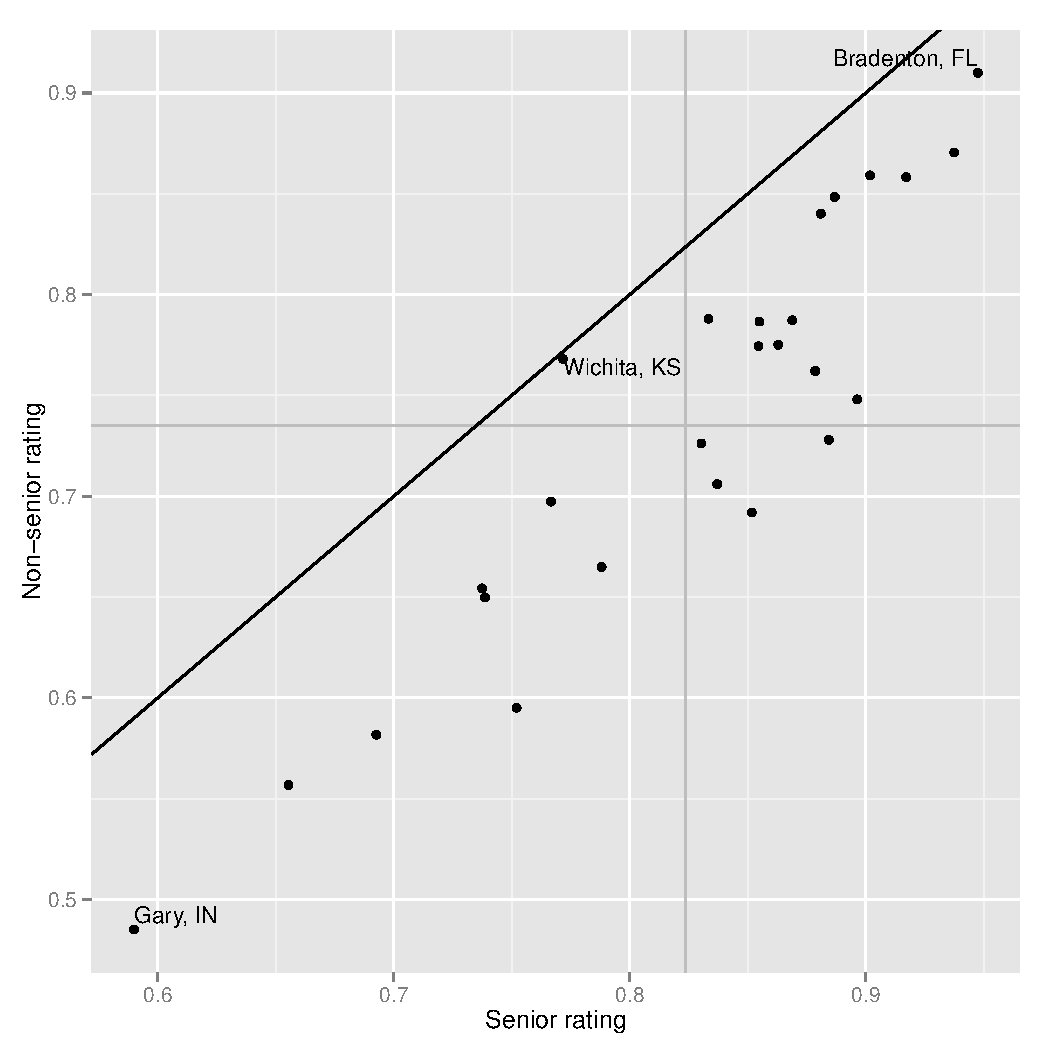
\includegraphics[width=0.76\linewidth]{anotherlookseniors-1} 

}

\caption[Relationship between positive responses to the question, ``How is your community as a place for seniors?" comparing ratings of non-seniors and seniors]{Relationship between positive responses to the question, ``How is your community as a place for seniors?" comparing ratings of non-seniors and seniors. The black line shows y=x, for comparison. Grey lines at x=0.82 and y=0.74 show the mean ratings by each group.}\label{fig:anotherlookseniors}
\end{figure}


\end{knitrout}

As in Section \ref{minorities}, we wanted to investigate the local variation in responses. To do this, a faceted plot of responses between the two groups was created. This plot can be seen in Figure \ref{fig:seniorPlot}, and it uses 2009 data. While this plot allows us to see the overall distribution of responses across communities, it makes it hard to compare the two groups (seniors and non-seniors) overall.

To see the relationship between total positive responses by non-seniors versus total positive responses by seniors to the question ``How is your community as a place for seniors?'' see Figure \ref{fig:anotherlookseniors}. Interestingly, every community followed the trend of non-seniors underestimating how good their community was for seniors (or seniors boosting their responses). The only community that came close to being an exception to this rule was Wichita, KS. There is a strong correlation between ratings both inside and outside the group ($r=$0.92), which suggests that there is good meta-knowledge about communities as places for seniors, although seniors always over-rate their communities. 

Then, the question becomes whether the $MK_S$ score is correlated with community satisfaction-- the value turns out to be \ensuremath{-0.11} This shows the relationship we would expect between community satisfaction and meta-knowledge, as communities with higher meta-knowledge also showed higher community satisfaction. 


\subsection{Meta-knowledge about the community as a place for families with young children}
The last subgroup to study in this exploration is families with young children. For this section, we split participants between those who reported having dependent children under the age of 18 living in their household and those who did not. Intuitively, it makes sense that a parent of an older child (say, a teenager) would have higher meta-knowledge about the community as a place for families with young children than a participant who never had children or whose children have grown up and moved away. While the data included more granular demographic details about the ages of the children in the households, splitting the data into participants with children and those without made the groups closer in size. To see the sample sizes and percentages, see Figure \ref{fig:kidsSS}. 



\begin{knitrout}
\definecolor{shadecolor}{rgb}{0.969, 0.969, 0.969}\color{fgcolor}\begin{figure}

{\centering 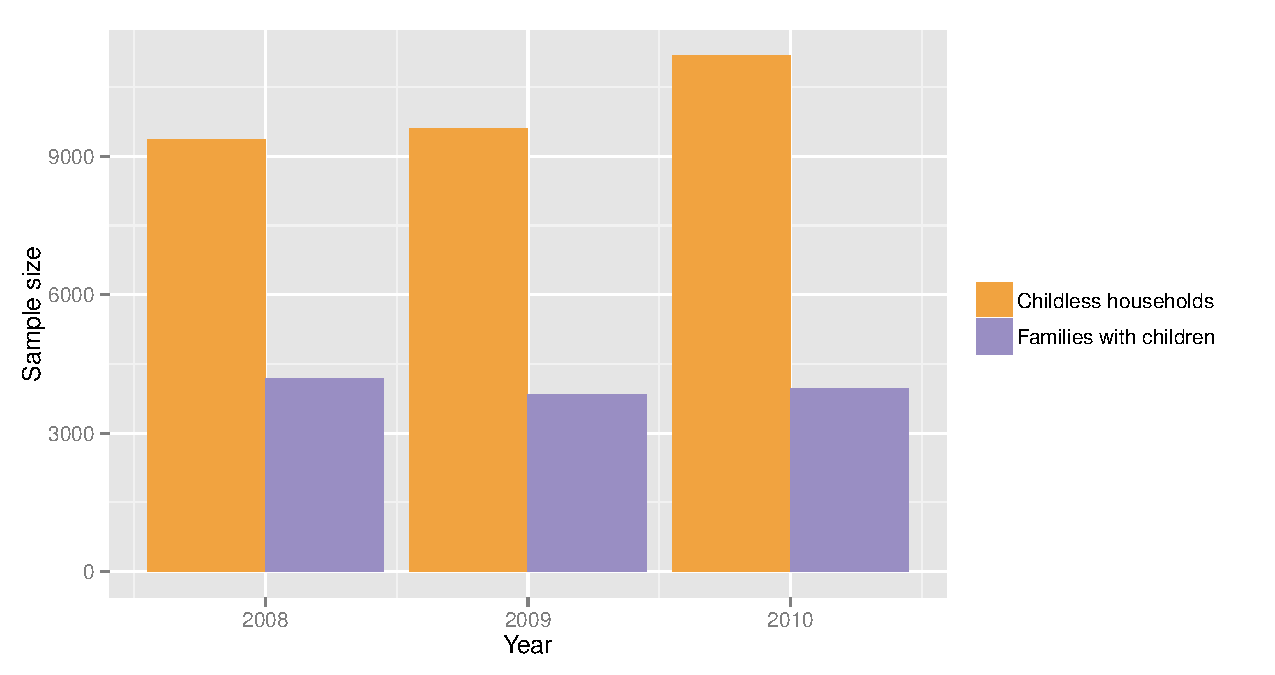
\includegraphics[width=0.99\linewidth]{kidsSS-1} 

}

\caption[Sample sizes for plots about meta-knowledge regarding the community as a place for families with young children]{Sample sizes for plots about meta-knowledge regarding the community as a place for families with young children.}\label{fig:kidsSS}
\end{figure}


\end{knitrout}



Figure \ref{fig:kidsplotOverall} shows the difference between the ratings of the groups over the three years of the survey. As in Section \ref{mseniors}, we can see that in-group ratings were slightly higher than out-group ratings, but the difference is not nearly as significant as in Section \ref{mseniors} on seniors. In fact, both groups seem to give about the same ratings overall. This shows that meta-knowledge about the community as a place for families with young children is generally high (that is, people without children have a good idea how their community is for families with children).

Again, we broke this down by community for the 2009 data, as seen in Figure \ref{fig:kidPlot}. Communities generally reflect the larger trend of good meta-knowledge outside the subgroup. To see the overall relationship between groups, we can look at Figure \ref{fig:anotherlookkids}. Communities generally reflect the larger trend of good meta-knowledge outside the subgroup. Accordingly, the variation apparent in Figure \ref{fig:kidPlot} is more about the overall ratings of the communities as places for raising kids. There was agreement both inside and outside the subgroup-- people seem to agree that State College, PA is a good place for families with young children, and Gary, IN and Macon, GA, are not. 

\begin{knitrout}
\definecolor{shadecolor}{rgb}{0.969, 0.969, 0.969}\color{fgcolor}\begin{figure}

{\centering 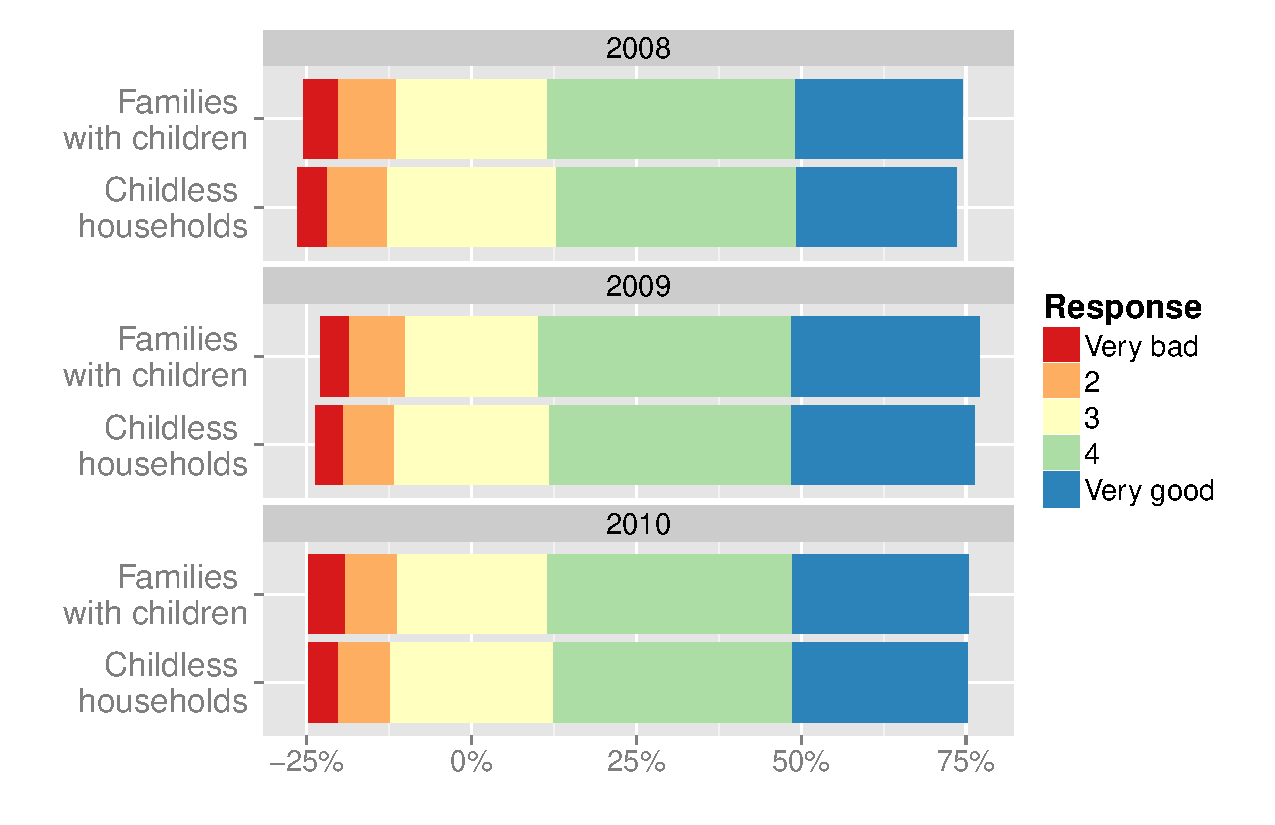
\includegraphics[width=0.99\linewidth]{kidsplotOverall-1} 

}

\caption[Responses to the question, ``How is your community as a place for families with young children?" Families with children are defined as any household with children under the age of 18, Childless households are any households without children, whether or not the residents have adult children living elsewhere]{Responses to the question, ``How is your community as a place for families with young children?" Families with children are defined as any household with children under the age of 18, Childless households are any households without children, whether or not the residents have adult children living elsewhere. Ratings were consistently similar between groups and across survey years.}\label{fig:kidsplotOverall}
\end{figure}


\end{knitrout}

\begin{knitrout}
\definecolor{shadecolor}{rgb}{0.969, 0.969, 0.969}\color{fgcolor}\begin{figure}

{\centering 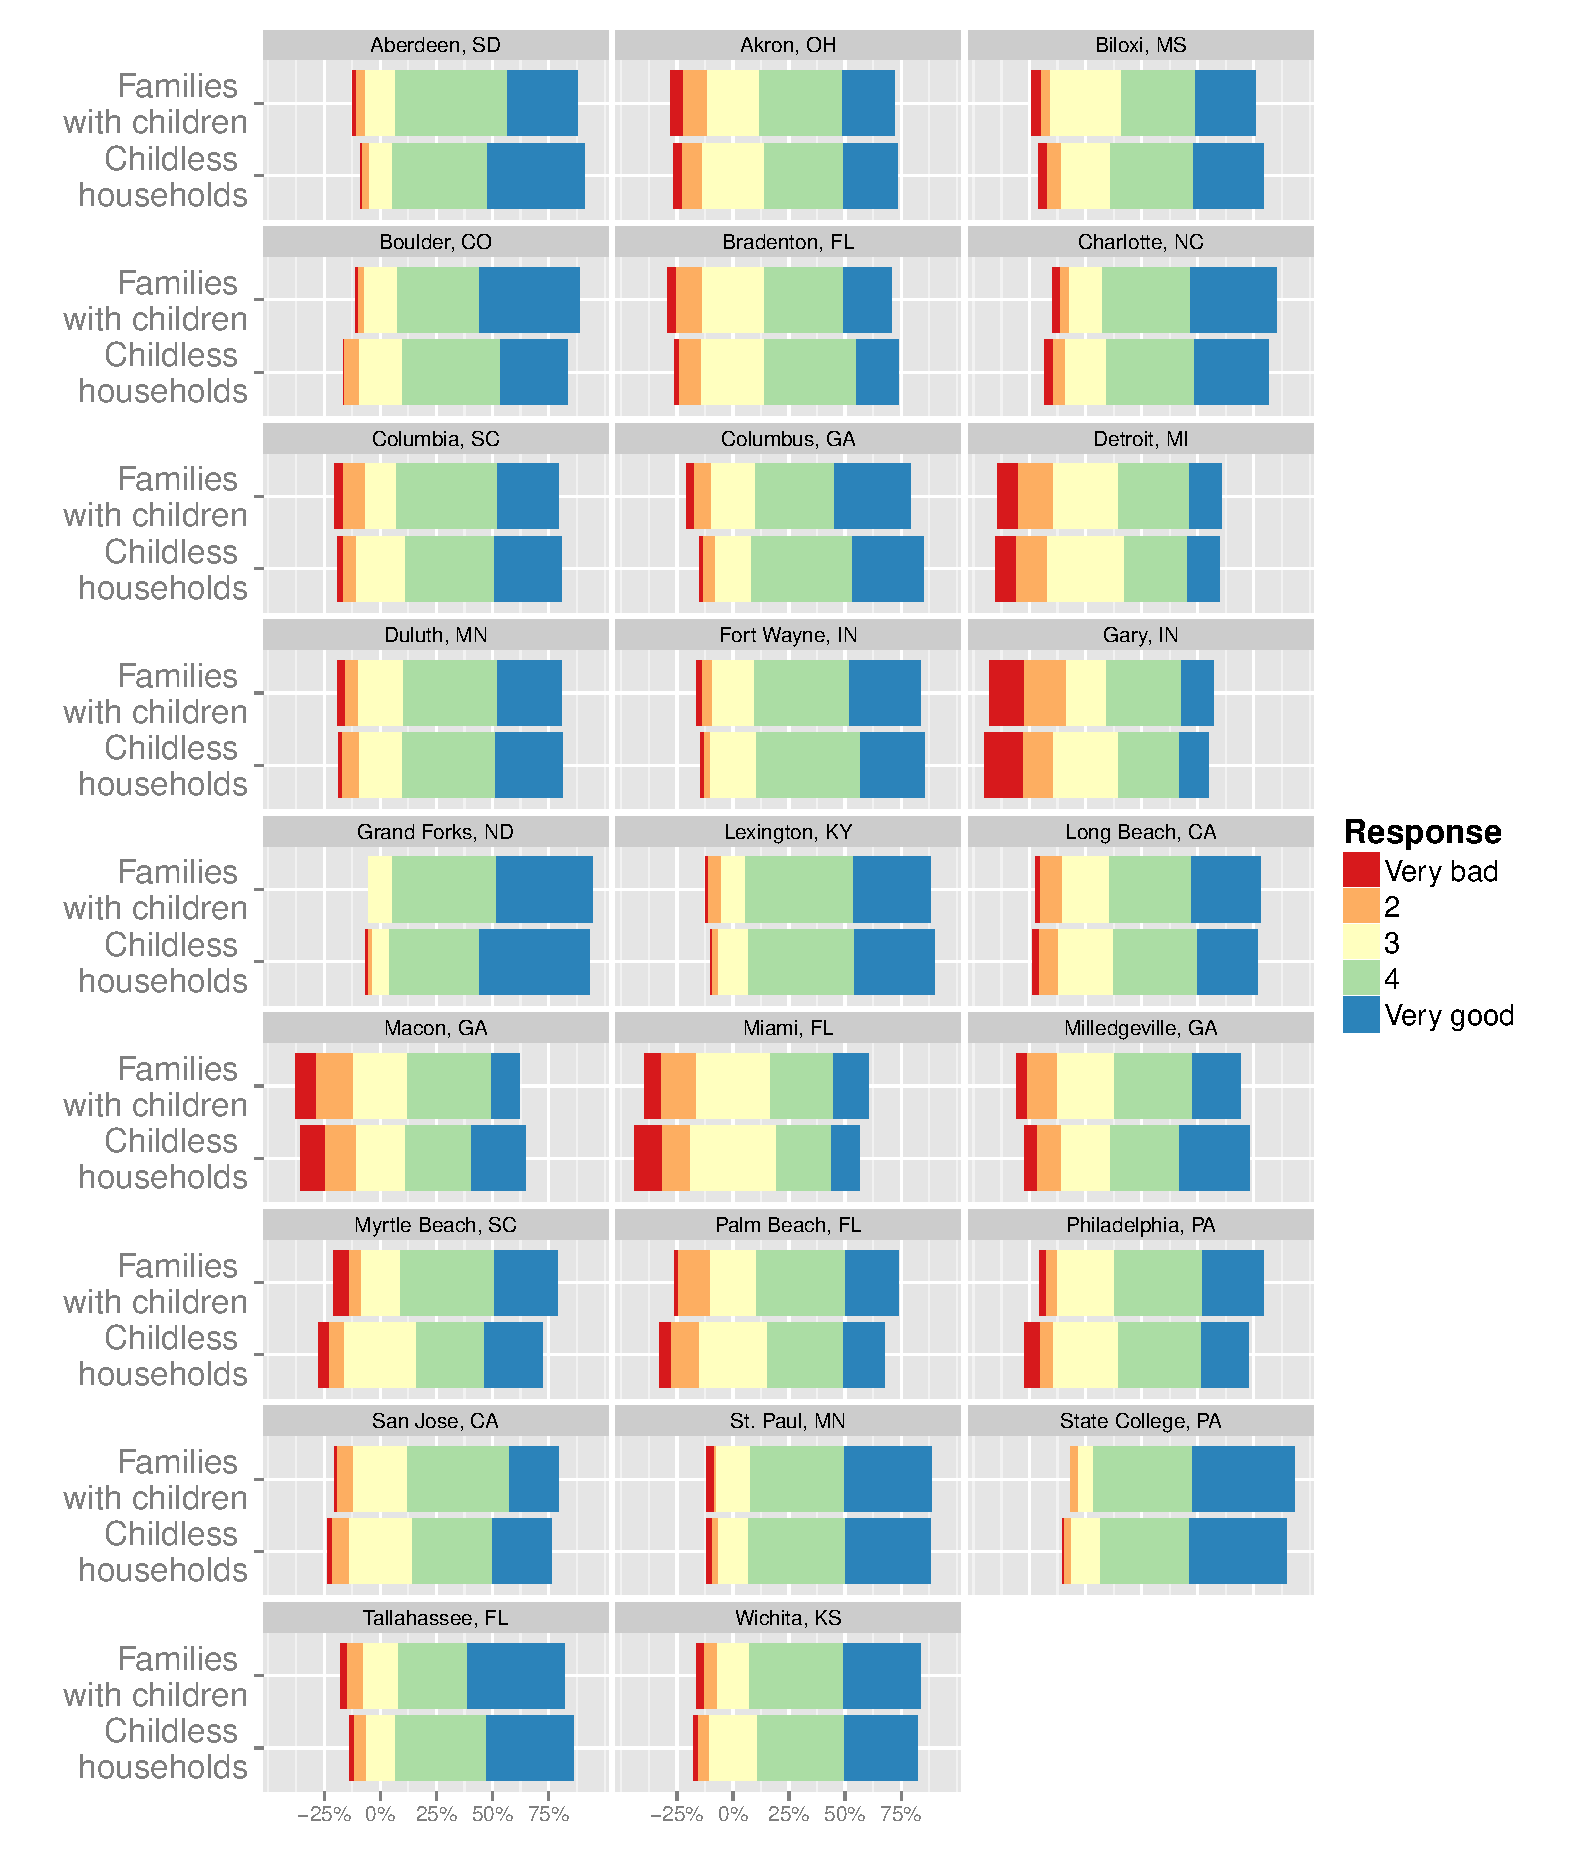
\includegraphics[width=0.99\linewidth]{kidPlot-1} 

}

\caption[Responses to the question, ``How is your community as a place for families with young children?" faceted by community (2009 data)]{Responses to the question, ``How is your community as a place for families with young children?" faceted by community (2009 data). Interestingly, most communities follow the pattern of similar ratings by both groups, but there is a lot of variation between communities in terms of the overall rating.}\label{fig:kidPlot}
\end{figure}


\end{knitrout}

\begin{knitrout}
\definecolor{shadecolor}{rgb}{0.969, 0.969, 0.969}\color{fgcolor}\begin{figure}

{\centering 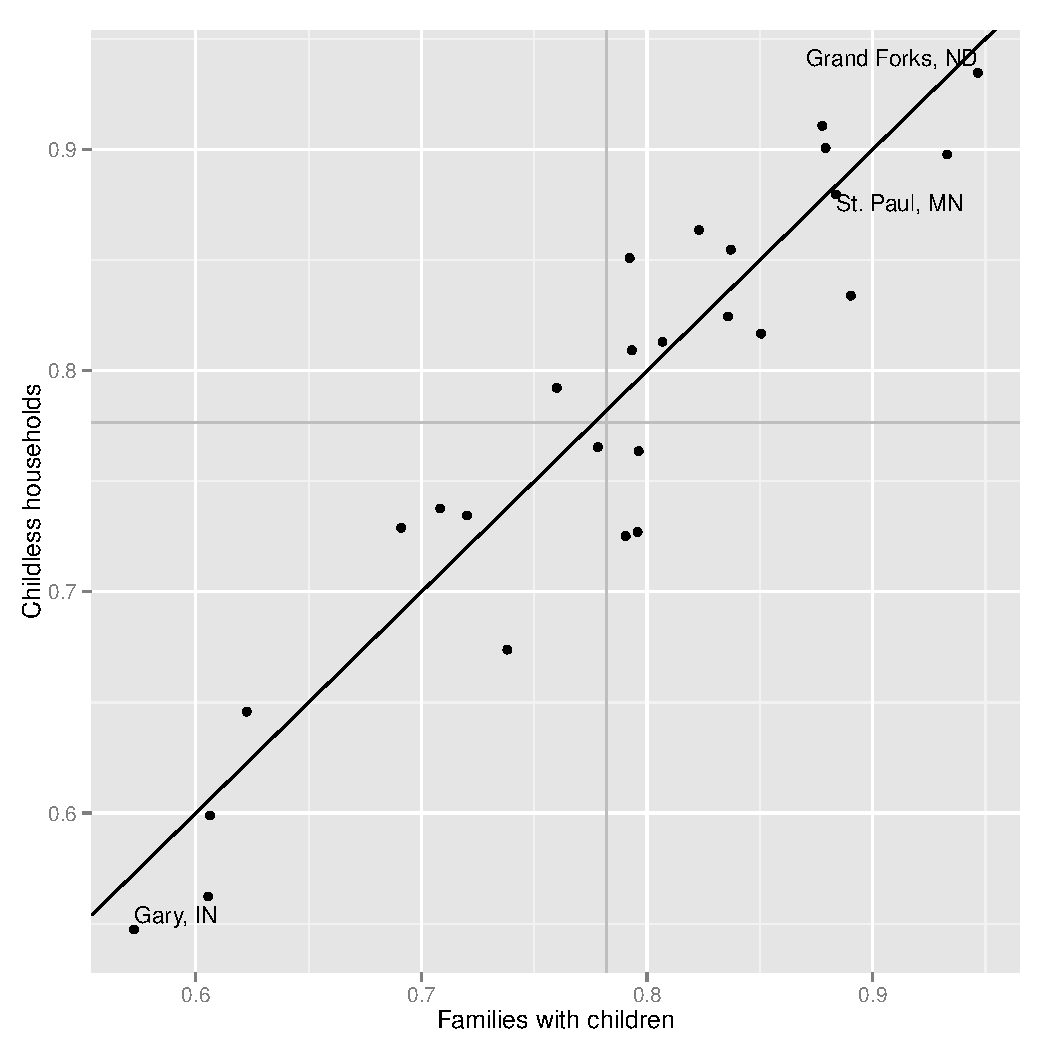
\includegraphics[width=0.76\linewidth]{anotherlookkids-1} 

}

\caption[Relationship between positive responses to the question, ``How is your community as a place for families with young children?" comparing ratings of families with kids and those without]{Relationship between positive responses to the question, ``How is your community as a place for families with young children?" comparing ratings of families with kids and those without. The black line shows y=x, for comparison. Grey lines at x=0.78 and y=0.78 show the mean ratings by each group.}\label{fig:anotherlookkids}
\end{figure}


\end{knitrout}

Finally, we can find the correlation between $MK_C$ and community satisfaction, $r= $\ensuremath{-0.16}. Again, this shows the direction of relationship we would expect-- larger community satisfaction scores are correlated with lower $MK_C$ scores. 

\subsection{Generalizing with meta-knowledge}
In order to further study the relationship between community satisfaction and meta knowledge, we want to be able to consider all three measures of meta-knowledge, $MK_R$, $MK_S$, and  $MK_C$, over all three years of data, and in conjunction with the measures of community engagement, like being registered to vote. 

The most obvious way to do this would be to fit some simple models, but because of the nature of the data (proportions of a population reporting community satisfaction), the coefficients soon become quite complex to interpret. Most modeling tasks either look to interpretability or predictive power, and in this case we are interested in interpretability. This is because the data does not even suggest causal links, so we cannot hope to modify one of the predictors and in turn influence the outcome. For example, consider the variable of seniors ratings of their community as a place for seniors. There is no way to artificially modify the way seniors think of their community as a place for seniors-- if you improve the community for them, you are likely to modify other aspects that people consider when thinking about community satisfaction. 

Instead of creating hard-to-interpret models, we simply consider more correlations between variables, looking at all three years. This can be seen in Figure \ref{fig:correlationmatrix}. 

\begin{knitrout}
\definecolor{shadecolor}{rgb}{0.969, 0.969, 0.969}\color{fgcolor}\begin{figure}

{\centering 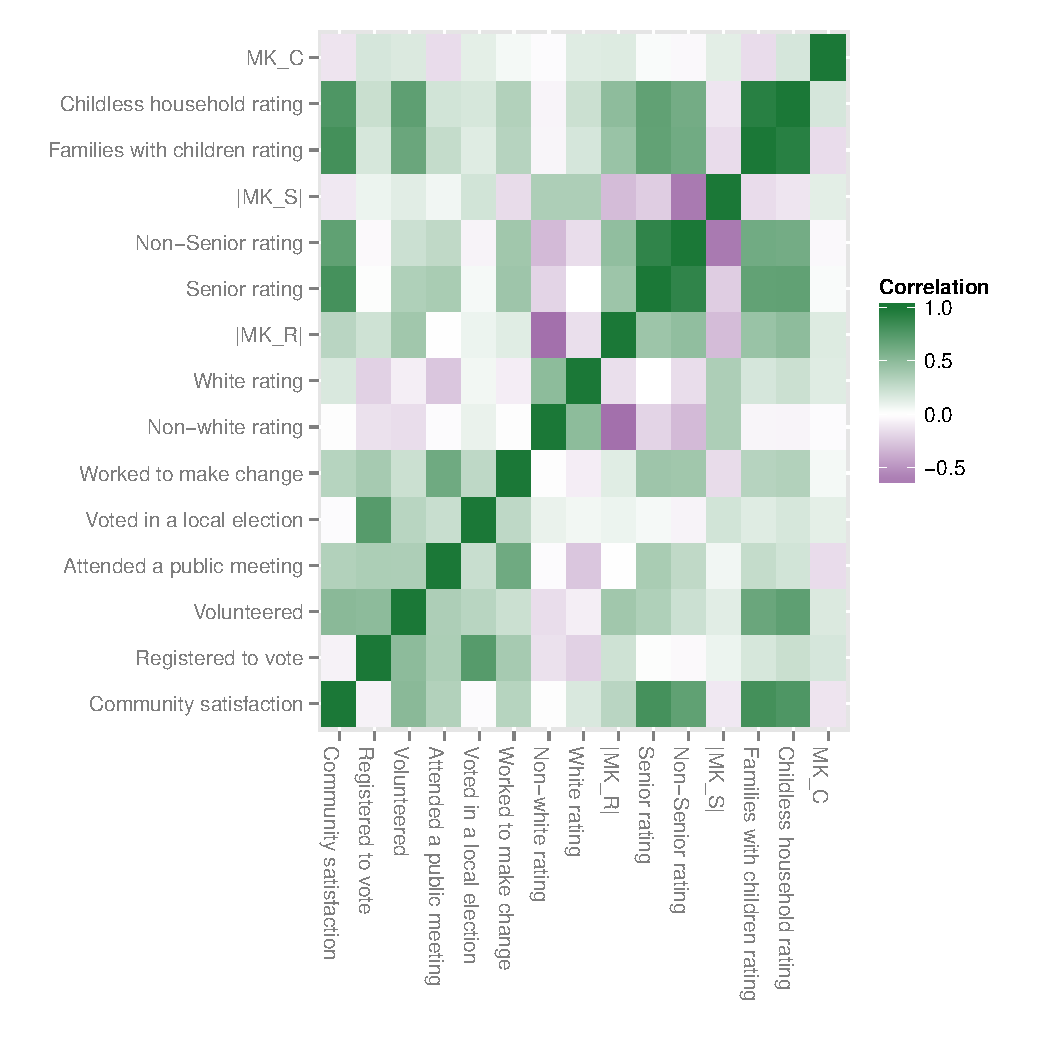
\includegraphics[width=\linewidth]{correlationmatrix-1} 

}

\caption[Correlation between variables of interest]{Correlation between variables of interest. In particular, look at the correlations of variables with Community Satisfaction. When reading the plot, recall that `[subgroup] rating` refers to their rating of their community as a place either for the associated minority group or the complement of that group in society, not to satisfaction overall. (2008, 2009, 2010 data, except for race-related questions where 2010 was excluded).}\label{fig:correlationmatrix}
\end{figure}


\end{knitrout}

There are many interesting insights which can be gleaned from this plot. The first is that there is typically a correlation between $MK$ score, and the scoring of the minority group that the score refers to. For example, there is a strong negative correlation between scoring of the community by Non-seniors and the $|MK_S|$ score. That is, communities where non-Seniors rated it as a good place for seniors, the difference between their ratings and seniors' ratings was smaller. 

There are also relationships between community engagement behaviors (for example, being registered to vote and voting in a local election) and between those engagement behaviors and meta-knowledge components (for example, ratings of the community as a place for families with young children and volunteering). 

These correlations suggest avenues for further study. 

\section{Conclusions and Further Work}
Through this exploration of the Knight Foundation's Soul of the Community data, we have been able to examine variability between communities and theorize about what might affect those variations. In Section \ref{communittsatsec} we saw which communities reported the highest levels of community satisfaction, namely State College, PA and Boulder, CO. In Section \ref{behaviorsec}, we explored the common behaviors that survey participants engaged in, including registering to vote and voting in local elections. We noticed that college towns tend to have higher than typical rates of providing shelter to a non-relative (the couchsurfing effect?).

Then, in Section \ref{metasec} we began to explore community meta-knowledge, or how aware survey participants are about their community as a place for minority groups. We explored meta-knowledge about how good a community is for racial and ethnic minorities, finding that there is a lot of variation between communities in whether minorities under- or over-rate their communities as a place for minorities, as compared to White respondents. There was some correlation between scores given by respondents in- and out-side the subgroup of racial and ethnic minorities, but not as strong as with the other facets of meta-knowledge. 

We noticed that non-seniors almost always under-rate how good their community is for seniors, but that there is a strong correlation between ratings by seniors and non-seniors, so the under-rating of the senior subgroup is simply a shift of an almost $y=x$ relationship. 

Communities also tend to have high meta-knowledge about how good their community is for families with young children (though there are exceptions). The relationship between respondents in- and out-side the subgroup was also linear and centered around $y=x$, with more variation both above and below. 

Through this exploration, we were able to expose variation between cities, years, and groups, but it is still not clear how useful this meta-knowledge could be as a measure of the soul of the community. 

In our final explorations, we studied the pattern of correlations between variables related to subgroup meta-knowledge and community engagement behaviors. Looking at these relationships, we were able to identify correlations that made intuitive sense (e.g. a correlation between being registered to vote and voting in a local election) as well as those that were un-intuitive (e.g. correlations between senior ratings about their community as a place for seniors and childless household ratings about the community as a place for families with young children). 

There are clearly deeper relationships at play here. It seems likely that there is a larger-scale measure of meta-knowledge that could be developed, taking into account more subgroups or transitions between groups. It would be interesting to explore whether seniors who had adult children had better meta-knowledge about their community as a place for families with young children, although they no longer exist in that particular subgroup. 
\bibliographystyle{plainnat}
\bibliography{SoCbib.bib}
\end{document}
